\documentclass{article}

\usepackage[paper=a4paper,margin=1.4in]{geometry}
\usepackage[OT1]{fontenc}
\usepackage{amsmath}
\usepackage[utf8]{inputenc}
\usepackage{amssymb}
\usepackage{amsxtra}
\usepackage{listings}
\usepackage{graphicx}
\usepackage[dvipsnames]{xcolor}
\usepackage{tikz,lipsum,lmodern}
\usepackage[most]{tcolorbox}
\usepackage{subcaption}
\usepackage[hidelinks]{hyperref}
\usepackage[shortlabels,inline]{enumitem}


\renewcommand*\familydefault{\sfdefault} % Set font to sans-serif
\graphicspath{ {figures/} }

\definecolor{highlight}{RGB}{29, 141, 176}

\newcommand{\refchapter}[1]{Chapter~\ref{#1}}
\newcommand{\refsec}[1]{Section~\ref{#1}}
\newcommand{\refeqn}[1]{Equation~(\ref{#1})}
\newcommand{\reffig}[1]{Figure~\ref{#1}}

% \newenvironment{task}[1]{
%   \begin{tcolorbox}[
%     colback=highlight!5!white,
%     colframe=highlight,
%     title={Task #1}
%   ]
% }{
%   \end{tcolorbox}
% }
\newenvironment{task}[1]{
  \subsubsection*{Task #1}
}{}

\title{
  \vspace*{2cm}
  {\bf \scriptsize
    KATHOLIEKE UNIVERSITEIT LEUVEN \\\vspace{0.3cm}
    Prof. Dr. ir. Johan A. K. Suykens
  } \vspace{2cm} \\
  Artificial Neural Networks \& Deep Learning \\
  {\large Exercise Reports}
}
\author{Marco Bischoff (R1012984)}

\begin{document}


\pagestyle{headings}

\maketitle
\newpage

\tableofcontents
\newpage



\section{Supervised Learning and Generalization}
\label{ex:1}


\setcounter{subsection}{2}
\subsection{In the Wide Jungle of the Training}
\label{ex:1.3}


\begin{task}{1.3.1}
  % What is the impact of the noise (parameter \texttt{noise} in the notebook) with respect to the
  % optimization process?
\end{task}

The noise parameter controls the deviation of the training data from the true function.
Figure~\ref{fig:ex1_noise-level} shows the impact of noise on the optimization process. For $noise =
  0$, the data exactly matches the true function and the model will converge to the true function
quickly. For $noise > 0$, the data is perturbed by noise and the model will take longer to converge.
For $noise = 1$, the data is completely random and the model will only converge to the mean of the
training data without being able to capture the underlying function.


\begin{task}{1.3.2}
  % How does (vanilla) gradient descent compare with respect to its stochastic and accelerated
  % versions?
\end{task}

Vanilla gradient descent is the slowest of the three methods. It computes the gradient of the loss
function for the entire training set at each iteration. Stochastic gradient descent (SGD) is faster
than vanilla gradient descent, because it computes the gradient for a random subset of the training
data at each iteration. However it has a higher variance in the loss function. Accelerated gradient
descent is the fastest of the three methods. It uses a momentum term to speed up convergence and
reduce oscillations in the loss function.


\begin{task}{1.3.3}
  % How does the size of the network impact the choice of the optimizer?
\end{task}

For small networks, vanilla gradient descent is sufficient, because the computation of the gradient
is not very expensive. For larger networks, SGD is more appropriate due to its lower computational
cost. Accelerated gradient descent is the best choice for very large networks, because it converges
faster than the other two methods.


\begin{task}{1.3.4}
  % Discuss the difference between epochs and time to assess the speed of the algorithms. What can it
  % mean to converge fast?
\end{task}

The model is trained for $2500$ epochs. In Figure~\ref{fig:ex1_optimizers}, we can see that SGD with
a learning rate of $0.05$ and without momentum has an average training time, but very slow
convergence. Using a learning rate of $0.1$ already converges much faster, but also takes longer to
compute. Momentum has a similar convergence rate and is much quicker to compute, but also has high
variance. The Adam and the LBFGS optimizers converge the fastest, but LBFGS has the longest
computational time. The Adam optimizer is the best choice for this problem, because it converges
quickly and has low variance. All optimizers except for vanilla SGD with learning rate $0.05$ can
be considered to have converged after at most $1000$ epochs.

\begin{figure}[ht!]
  \centering
  \begin{minipage}{0.48\textwidth}
    \centering
    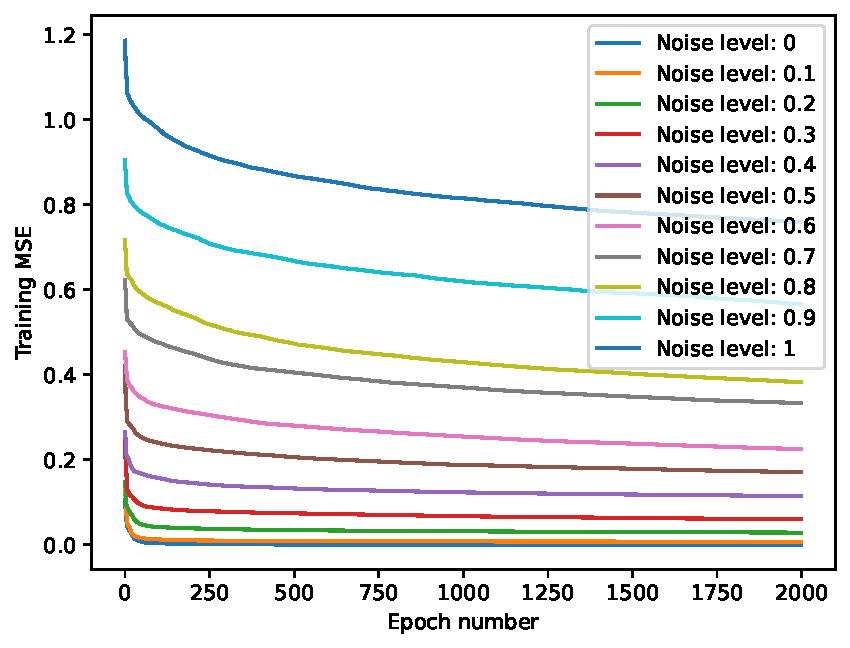
\includegraphics[width=0.9\linewidth]{ex1_noise-level.pdf}
    \captionof{figure}{Impact of noise on the optimization process}
    \label{fig:ex1_noise-level}
  \end{minipage}
  \begin{minipage}{0.48\textwidth}
    \centering
    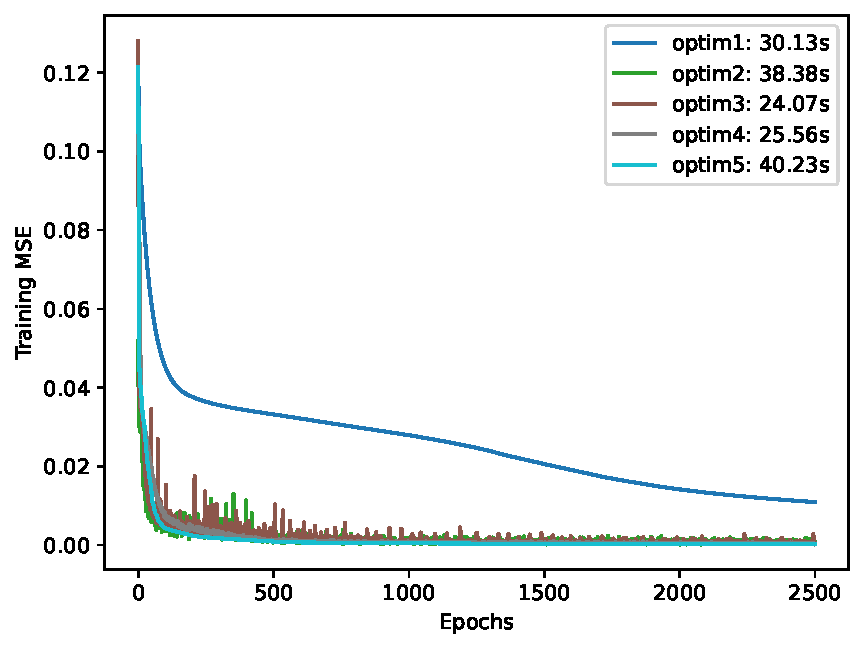
\includegraphics[width=0.9\linewidth]{ex1_optimizers.pdf}
    \captionof{figure}{Comparison of optimizers}
    \label{fig:ex1_optimizers}
  \end{minipage}
\end{figure}


\subsubsection*{A bigger model}
\begin{task}{1.3.5}
  % How many parameters does the model have?
\end{task}

The model has $34826$ parameters in total as shown in Table~\ref{tab:ex1_model}.

\begin{table}[ht!]
  \begin{tabular}{|l|l|r|}
    \hline
    \textbf{Layer Type} & \textbf{Shape} & \textbf{\# Param} \\ \hline
    (Input)             & (28, 28, 1)    & 0                 \\ \hline
    Conv2D              & (26, 26, 32)   & 320               \\ \hline
    MaxPooling2D        & (13, 13, 32)   & 0                 \\ \hline
    Conv2D              & (11, 11, 64)   & 18496             \\ \hline
    MaxPooling2D        & (5, 5, 64)     & 0                 \\ \hline
    Flatten             & (1600, )       & 0                 \\ \hline
    Dropout             & (1600, )       & 0                 \\ \hline
    Dense               & (10, )         & 16010             \\ \hline\hline
    \textbf{Total}      &                & \textbf{34826}    \\ \hline
  \end{tabular}
  \centering
  \caption{Model parameters}
  \label{tab:ex1_model}
\end{table}


\begin{task}{1.3.6}
  % Replace the ADAM optimizer by a SGD one. Can you still achieve excellent performances? Try then
  % the Adadelta optimizer. What is its particularity?
\end{task}

The SGD optimizer has a much slower convergence rate than the Adam optimizer as shown in
Figure~\ref{fig:ex1_mnist_optimizers}. The Adadelta optimizer achieves very good performance after
the first epoch already and has a low variance. The Adam optimizer is in between the two in
terms of convergence rate and variance. Compared to the Adam optimizer, the Adadelta optimizer
does not require a learning rate to be set, because it uses the gradient and the average of
the squared gradient over a window of time steps to adapt the learning rate.



\subsection{A Personal Regression Exercise}
\label{ex:1.4}

\begin{task}{1.4.1}
  % Define your training and testing dataset using respectively 2000 and 1000 samples drawn
  % independently. Explain the point of having different datasets for training and testing. Plot the
  % surface associated to the training set.
\end{task}

\begin{figure}[ht!]
  \centering
  \begin{minipage}{0.48\textwidth}
    \centering
    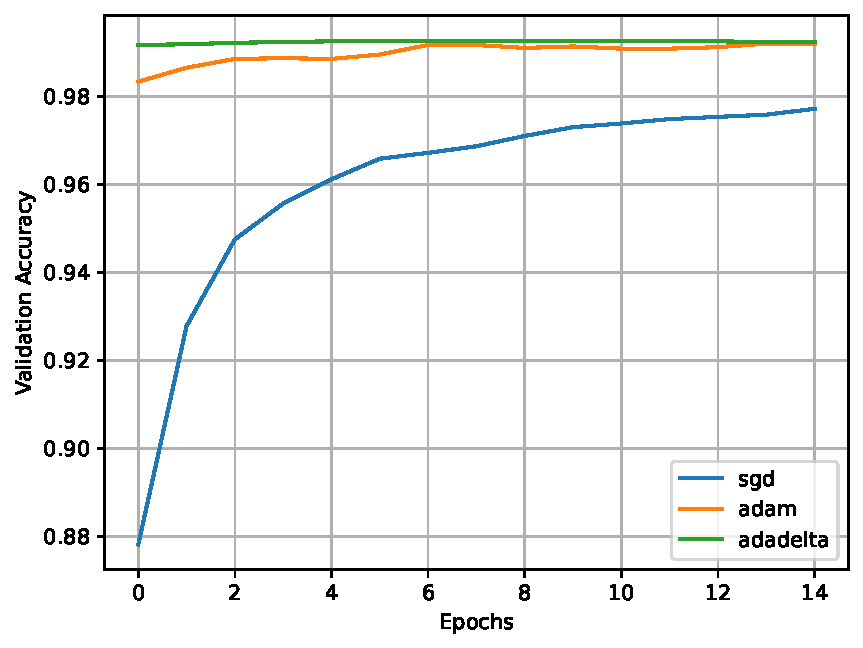
\includegraphics[width=0.9\linewidth]{ex1_mnist_optimizers.pdf}
    \captionof{figure}{Validation accuracy}
    \label{fig:ex1_mnist_optimizers}
  \end{minipage}
  \begin{minipage}{0.48\textwidth}
    \centering
    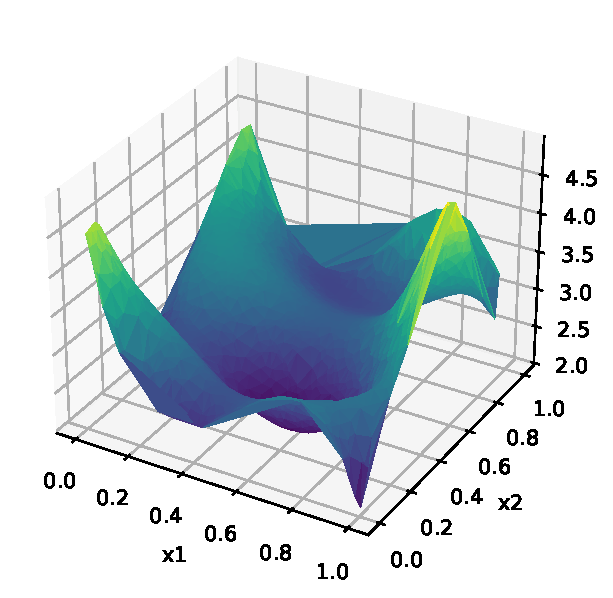
\includegraphics[width=0.9\linewidth]{ex1_regression_train.pdf}
    \captionof{figure}{Function surface of the training data}
    \label{fig:ex1_regression_train}
  \end{minipage}
\end{figure}

If the same dataset is used for training and testing, the model will overfit the data and not
generalize well to unseen data. Moreover, the evaluation of the model will be biased, because the
model has already seen the test data during training. If two independent datasets are used, the
performance on the test data corresponds more to real-world performance, where the model has not
seen the data before. Also, the performance on the test data will be bad, if the model has overfit
the training data. The surface associated to the training set is shown in
Figure~\ref{fig:ex1_regression_train}.


\begin{task}{1.4.2}
  % Build and train your feedforward neural network. To that end, you must perform an adequate model
  % selection on the training set. Investigate carefully the architecture of your model: number of
  % layers, number of neurons, learning algorithm and transfer function. How do you validate your
  % model?
\end{task}

The model architecture is shown in Table~\ref{tab:ex1_regression_model}. The choice of the
activation functions seemed to have the biggest impact on the performance. The \texttt{mish}
activation function performed much better than the other functions I tried. Increasing the number of
layers and neurons also improved the performance. However, the model was overfitting the training
data when using too many neurons. The choice of the optimizer and the learning rate did not have a
big impact on the performance. Here, I used the Adam optimizer with a learning rate of $0.05$. All
choices were validated by calculating the mean squared error on the test data.

\begin{table}[ht!]
  \centering
  \begin{tabular}{|l|l|l|r|}
    \hline
    \textbf{Layer Type} & \textbf{Shape} & \textbf{Activation Function} & \textbf{\# Param} \\ \hline
    Dense               & (16)           & mish                         & 48                \\ \hline
    Dense               & (16)           & mish                         & 272               \\ \hline
    Dense               & (16)           & tanh                         & 272               \\ \hline
    Dense               & (1)            & (None)                       & 17                \\ \hline\hline
    \textbf{Total}      &                &                              & \textbf{609}      \\ \hline
  \end{tabular}
  \caption{Regression model parameters}
  \label{tab:ex1_regression_model}
\end{table}


\begin{task}{1.4.3}
  % Evaluate the performance of your selected network on the test set. Plot the surface of the test
  % set and the approximation given by the network. Explain why you cannot train further. Give the
  % final MSE on the test set.
\end{task}

The surfaces of the test data and the predicted data are shown in
Figure~\ref{fig:ex1_regression_surface}. The model has already converged and further training would
not improve the performance. The final mean squared error on the test data is $0.0017132$.

\begin{figure}[ht!]
  \centering
  \begin{subfigure}{0.49\textwidth}
    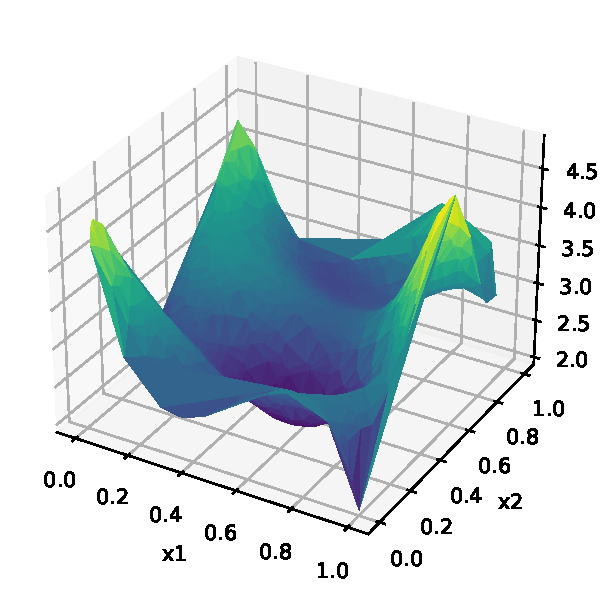
\includegraphics[width=\textwidth]{ex1_regression_test.pdf}
    \caption{Test data}
    \label{fig:ex1_regression_test}
  \end{subfigure}
  \begin{subfigure}{0.49\textwidth}
    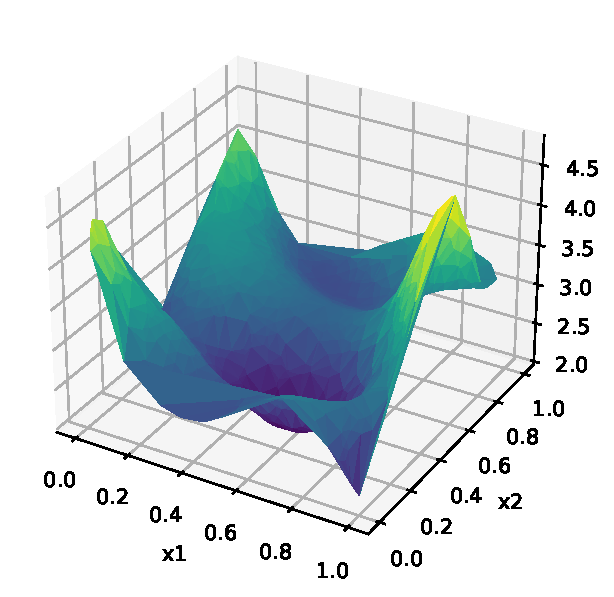
\includegraphics[width=\textwidth]{ex1_regression_predicted.pdf}
    \caption{Predicted}
    \label{fig:ex1_regression_predicted}
  \end{subfigure}
  \caption{Function surface}
  \label{fig:ex1_regression_surface}
\end{figure}


\begin{task}{1.4.4}
  % Describe the regularization strategy that you used to avoid overfitting. What other strategy can you
  % think of?
\end{task}

I used early stopping to avoid overfitting. The training was stopped when the validation loss did
not improve for $10$ epochs. Another strategy to avoid overfitting is to use dropout layers, which
sets a few neurons to zero during training.


\section{Recurrent Neural Networks}
\label{ex:2}


\subsection{Hopfield Networks}
\label{ex:2.1}


\begin{task}{2.1.1}
  % Create a Hopfield network with target patterns $[1, 1]$, $[-1, -1]$ and $[1, -1]$ and the
  % corresponding number of neurons. Simulate the state evolution for various input vectors (e.g.
  % random points or points of high symmetry) and note down the obtained attractors after a
  % sufficient number of iterations. Are the real attractors the same as those used to create the
  % network? If not, why do we get these unwanted attractors? How many iterations does it typically
  % take to reach the attractor? What can you say about the stability of the attractors?
\end{task}

All of the attractor states $[1, 1]$, $[-1, -1]$ and $[1, -1]$ are reached after a few iterations,
as shown in Figure~\ref{fig:ex2_1_2D_random}. We also get the unwanted attractor $[-1, 1]$ because
the network is not able to distinguish between the patterns $[1, -1]$ and $[-1, 1]$. The ten random
points in Figure~\ref{fig:ex2_1_2D_random} converged after an average of $8.6$ iterations. The
attractors are stable, as further iterations do not change the state of the network. However, if
initial points are placed exactly in the middle between two attractors, they stay unaffected by
updates, as shown in Figure~\ref{fig:ex2_1_2D_edge}. These points are additional attractors, which
are not part of the target patterns. They are unstable, as small perturbations will make the network
converge to one of the stable attractors.

\begin{figure}[ht!]
  \centering
  \begin{subfigure}{0.49\textwidth}
    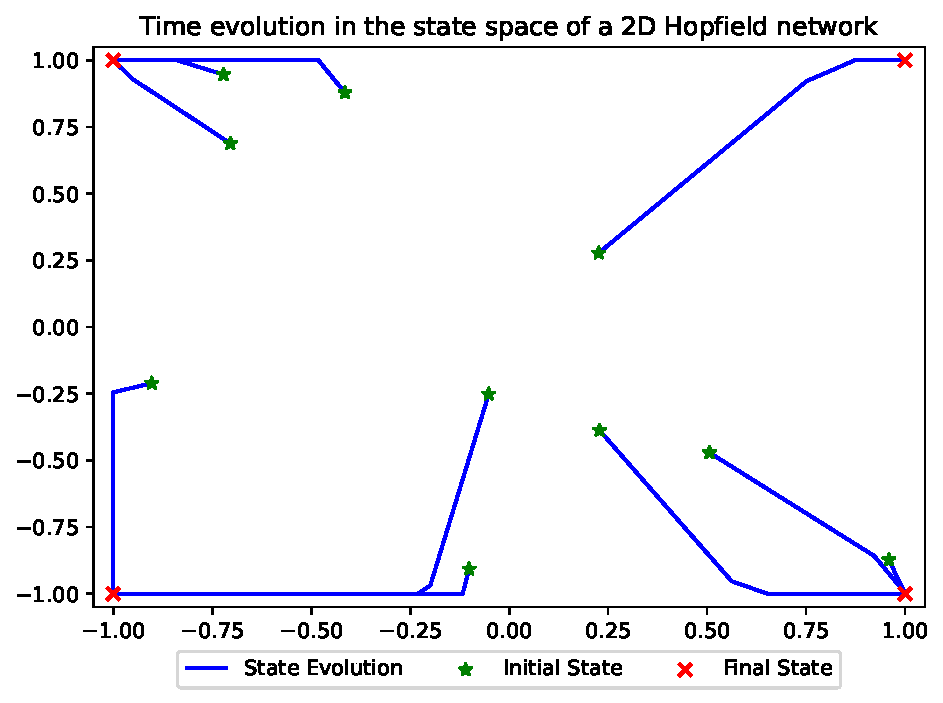
\includegraphics[width=\textwidth]{ex2_1_hopfield2D.pdf}
    \label{fig:ex2_1_hopfield2D}
  \end{subfigure}
  \begin{subfigure}{0.49\textwidth}
    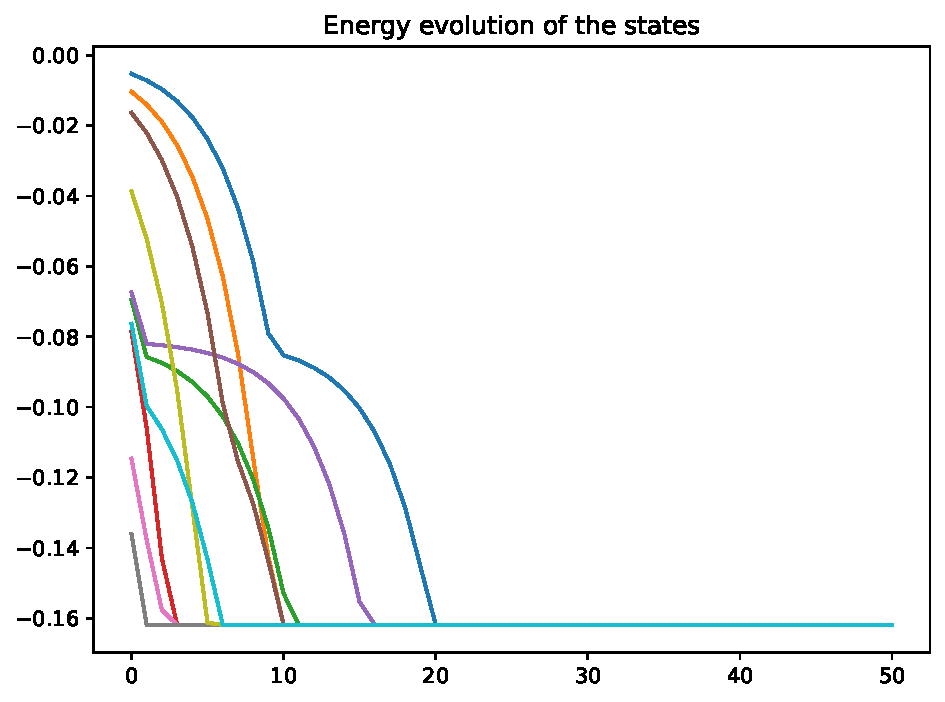
\includegraphics[width=\textwidth]{ex2_1_energy2D.pdf}
    \label{fig:ex2_1_energy2D}
  \end{subfigure}
  \caption{2D network: random inputs}
  \label{fig:ex2_1_2D_random}
\end{figure}

\begin{figure}[ht!]
  \centering
  \begin{subfigure}{0.49\textwidth}
    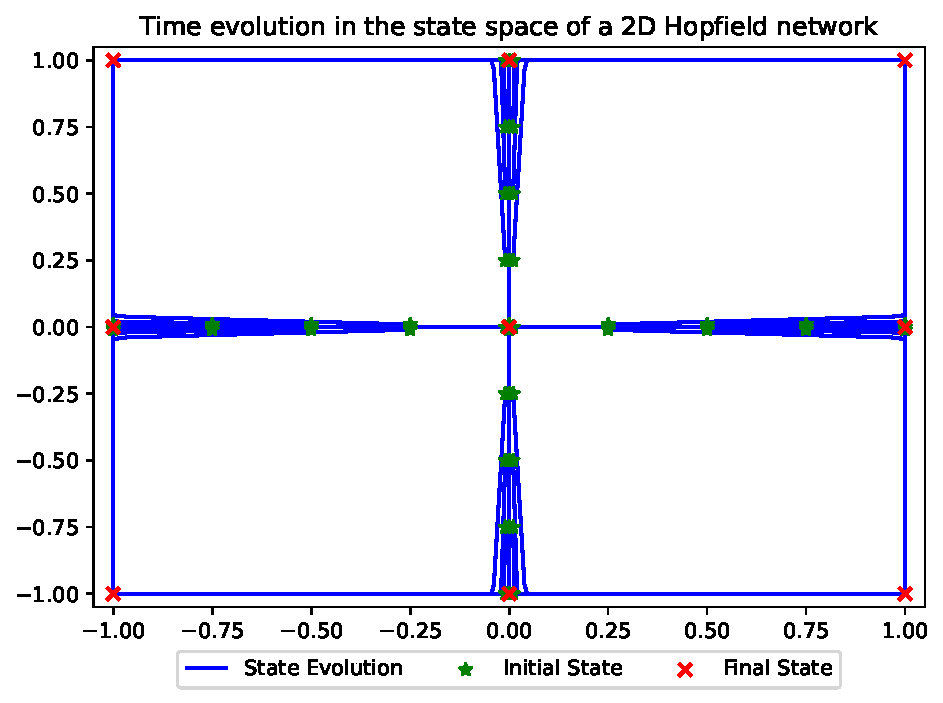
\includegraphics[width=\textwidth]{ex2_1_hopfield2D_edge.pdf}
    \label{fig:ex2_1_hopfield2D_edge}
  \end{subfigure}
  \begin{subfigure}{0.49\textwidth}
    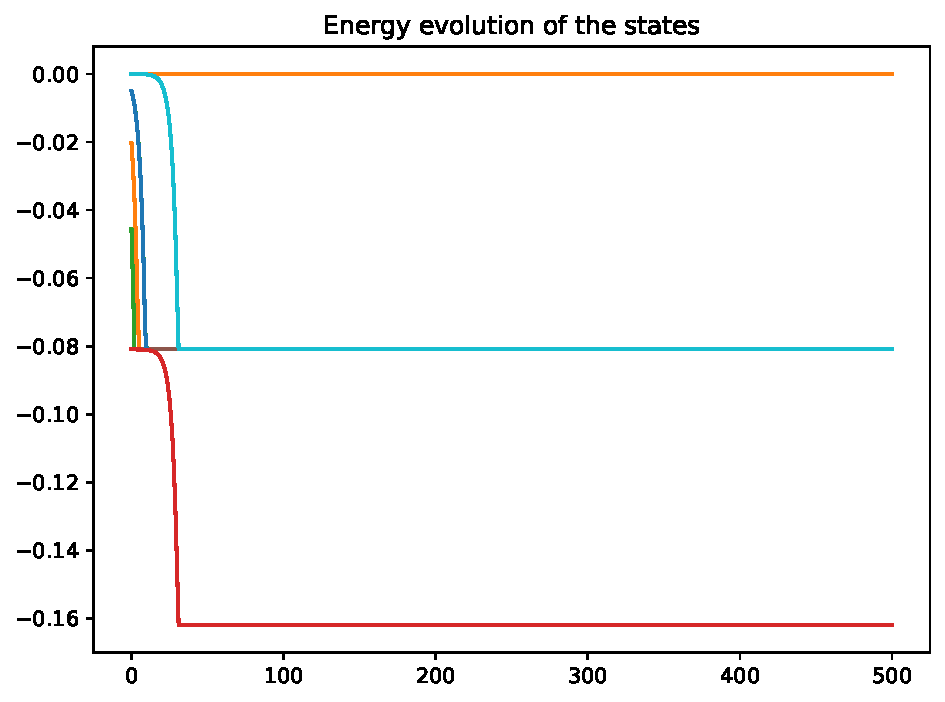
\includegraphics[width=\textwidth]{ex2_1_energy2D_edge.pdf}
    \label{fig:ex2_1_energy2D_edge}
  \end{subfigure}
  \caption{2D network: inputs close to local minima}
  \label{fig:ex2_1_2D_edge}
\end{figure}



\begin{task}{2.1.2}
  % Do the same for a three neuron Hopfield network, this time for the target patterns $[1, 1, 1]$,
  % $[-1, -1, 1]$ and $[1, -1, -1]$.
\end{task}

For the 3D network, all the target patterns $[1, 1, 1]$, $[-1, -1, 1]$ and $[1, -1, -1]$ are
reached, as shown in Figure~\ref{fig:ex2_1_3D_random}. No additional attractors are found. The
average number of iterations is $11.7$. All of the attractors are stable, even if the initial points
are placed exactly in the middle between two attractors, as shown in Figure~\ref{fig:ex2_1_3D_edge}.
The simulated points first move towards the plane that goes through all three attractors, and then
moves along this plane to the closest attractor.

\begin{figure}[ht!]
  \centering
  \begin{subfigure}{0.49\textwidth}
    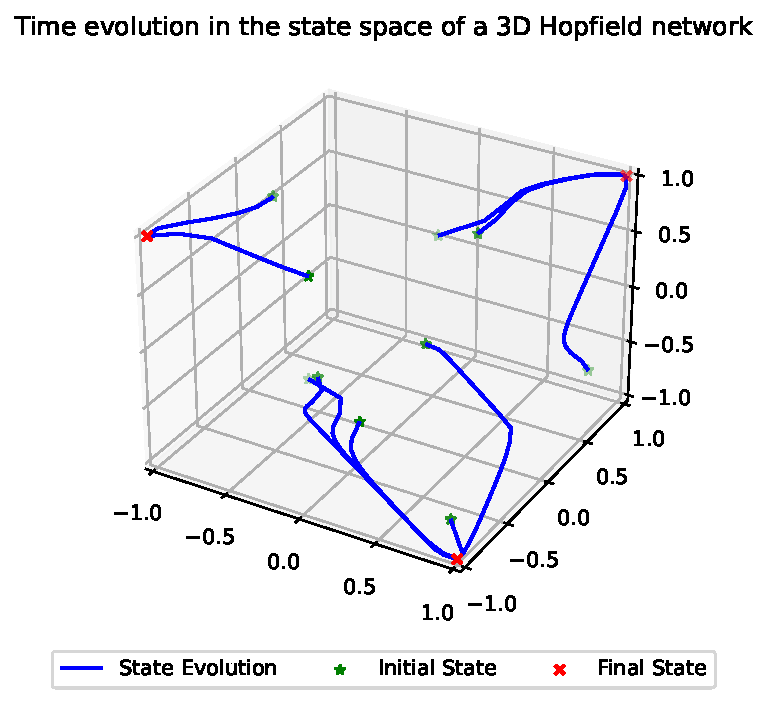
\includegraphics[width=\textwidth]{ex2_1_hopfield3D.pdf}
    \label{fig:ex2_1_hopfield3D}
  \end{subfigure}
  \begin{subfigure}{0.49\textwidth}
    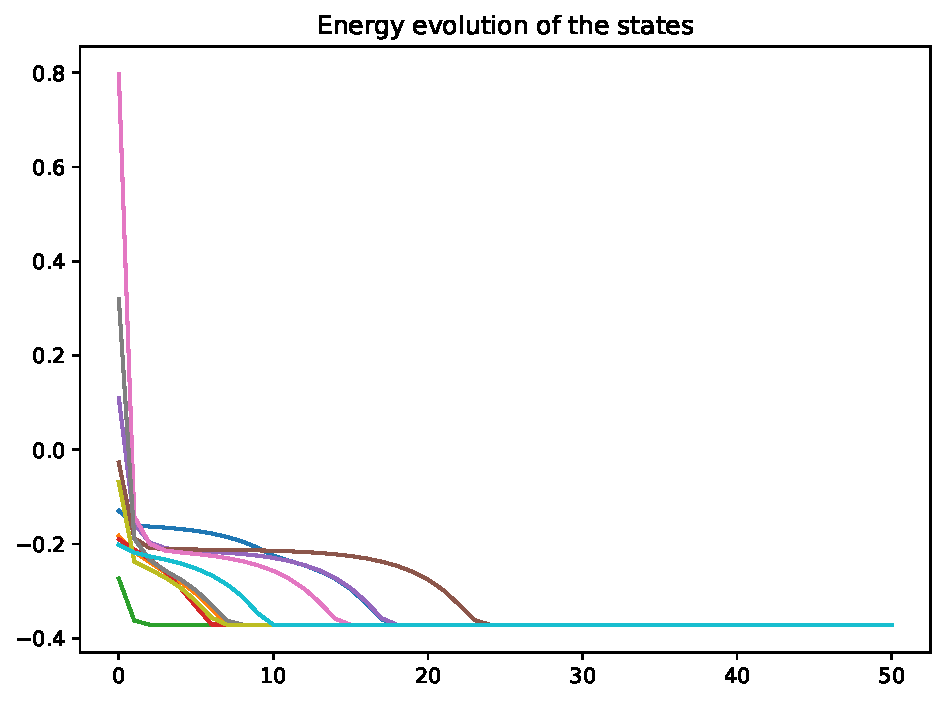
\includegraphics[width=\textwidth]{ex2_1_energy3D.pdf}
    \label{fig:ex2_1_energy3D}
  \end{subfigure}
  \caption{3D network: random inputs}
  \label{fig:ex2_1_3D_random}
\end{figure}

\begin{figure}[ht!]
  \centering
  \begin{subfigure}{0.49\textwidth}
    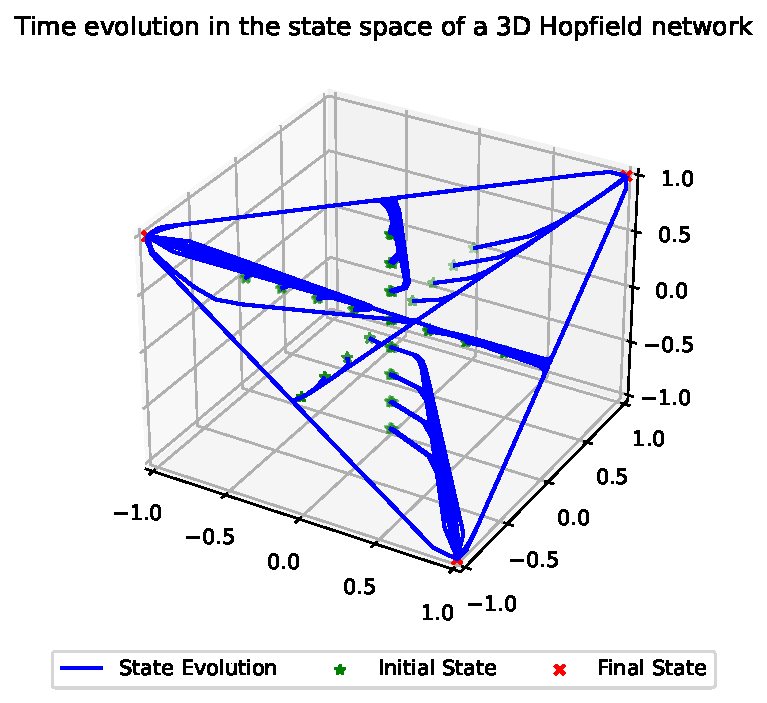
\includegraphics[width=\textwidth]{ex2_1_hopfield3D_edge.pdf}
    \label{fig:ex2_1_hopfield3D_edge}
  \end{subfigure}
  \begin{subfigure}{0.49\textwidth}
    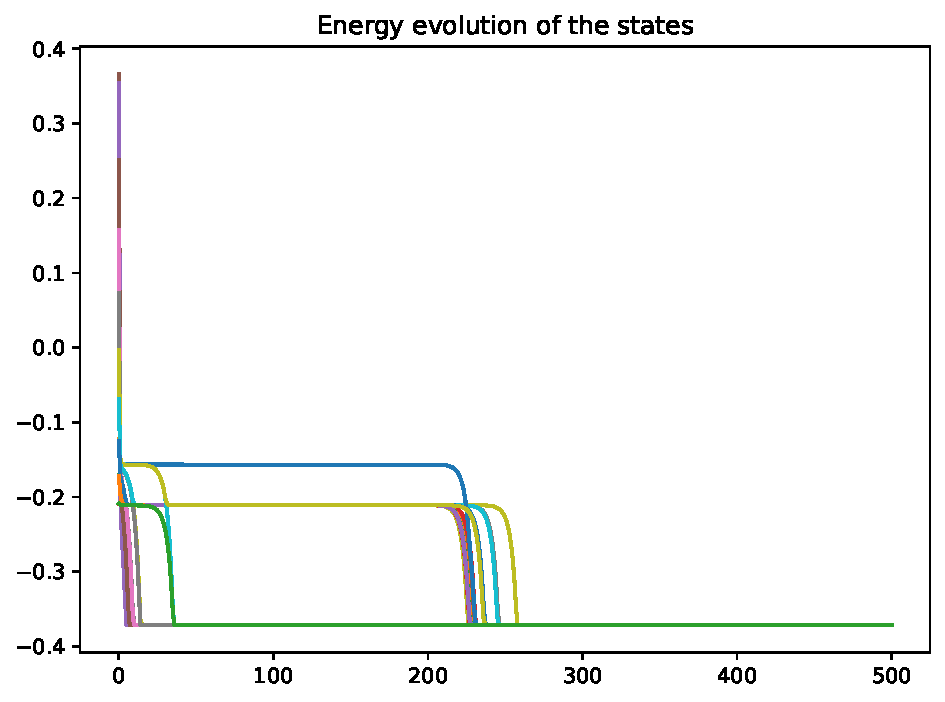
\includegraphics[width=\textwidth]{ex2_1_energy3D_edge.pdf}
    \label{fig:ex2_1_energy3D_edge}
  \end{subfigure}
  \caption{3D network: inputs close to local minima}
  \label{fig:ex2_1_3D_edge}
\end{figure}



\begin{task}{2.1.3}
  % Create a higher dimensional Hopfield network which has as attractors the handwritten digits from
  % 0 to 9. Test the ability of the network to correctly retrieve these patterns when some noisy
  % digits are given as input to the network. Try to answer the below questions by playing with
  % these two parameters:
  % \begin{itemize}
  %   \item \texttt{noise level} represents the level of noise that will corrupt the digits and is
  %         a positive number.
  %   \item \texttt{num iter} is the number of iterations the Hopfield network (having as input the
  %         noisy digits) will run.
  % \end{itemize}
  % Is the Hopfield model always able to reconstruct the noisy digits? If not why? What is the
  % influence of the noise on the number of iterations?
\end{task}

For $100$ iterations, the network is able to reconstruct the noisy digits for noise levels up to
$5$. Above this level, a few digits converge to the wrong attractor. Some digits are less robust to
noise than others. For example, the digit $7$ is often reconstructed as a $3$. Also, with less
iterations, the network often does not fully converge to an attractor. This leaves traces of the
noisy input in the reconstructed digit. For a good reconstruction with a noise level of $5$, the
number of iterations should be at least $40$. For a noise level of $1$, the network is able to
converge after only $4$ iterations.


\subsection{Timeseries Prediction}
\label{ex:2.2}


\begin{task}{2.2.1}
  % Train an MLP with one hidden layer. Investigate the model performance with different lags and
  % number of neurons. Discuss how the model looks and explain clearly how you tune the parameters
  % and what the influence on the final prediction is. Which combination of parameters gives the
  % best performance (MSE) on the test set?
\end{task}



\begin{task}{2.2.2}
  % Do the same for the LSTM model and explain the design process. What is the effect of changing
  % the lag value for the LSTM network?
\end{task}



\begin{task}{2.2.3}
  % Compare the results of the recurrent MLP with the LSTM. Which model do you prefer and why?
\end{task}


\section{Deep Feature Learning}
\label{ex:3}


\subsection{Stacked Autoencoders}
\label{ex:3.1}

\begin{task}{3.1.1}
  % Conduct image classification on MNIST using an stacked autoencoder. Are you able to obtain a
  % better result by changing the size of the network architecture? What are the results before and
  % after fine-tuning? What is the benefit of pretraining the network layer by layer?
\end{task}

I am using two autoencoders stacked on top of each other with hidden dimensions $256$ and $64$
respectively. Changing the size of the network architecture did not yield significant improvements.
Changing the number of epochs however did. I got the best results with $20$ epochs for pre-training
each layer, $30$ epochs to train the classification layer and $50$ epochs to fine-tune the whole
network. The loss for every training step is shown in Figure~\ref{fig:ex3_1_loss}. Fine-tuning
significantly improved the performance. The accuracy on the test set was $0.955$. Pretraining the
network layer by layer helps to find a good initialization for the weights. This seems to work
well in this case. However, the network was not able to learn by training the classification layer.

\begin{figure}[ht!]
  \centering
  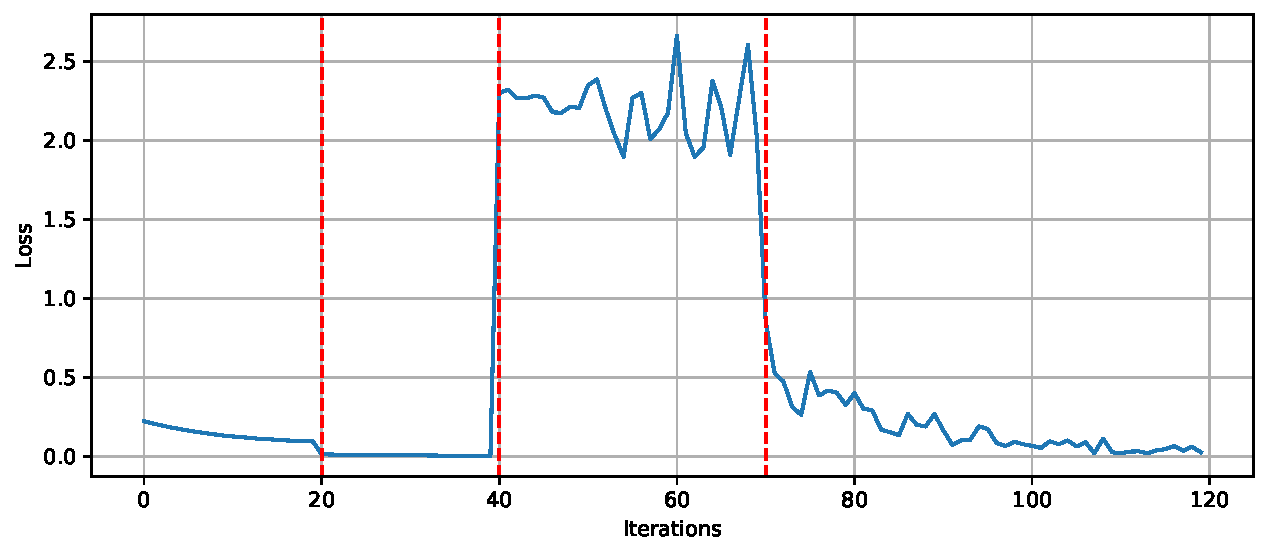
\includegraphics[width=0.9\textwidth]{ex3_1_loss.pdf}
  \caption{Loss for the stacked autoencoder. (1) Pre-training the first layer, (2) pre-training the
    second layer, (3) training the classification layer, (4) fine-tuning the whole network.}
  \label{fig:ex3_1_loss}
\end{figure}

% WITH epochs = (10, 10, 20)
% hidden_dim1 = 256
% hidden_dim2 = 64
% -> Accuracy on the test set: 0.918, last loss: 0.1718
% hidden_dim1 = 128
% hidden_dim2 = 32
% -> Accuracy on the test set: 0.924, last loss: 0.1339
% hidden_dim1 = 128
% hidden_dim2 = 64
% -> Accuracy on the test set: 0.916, last loss: 0.2189
% hidden_dim1 = 64
% hidden_dim2 = 16
% -> Accuracy on the test set: 0.923, last loss: 0.1196
% hidden_dim1 = 64
% hidden_dim2 = 32
% -> Accuracy on the test set: 0.937, last loss: 0.1227
% hidden_dim1 = 32
% hidden_dim2 = 16
% -> Accuracy on the test set: 0.923, last loss: 0.0933
% hidden_dim1 = 32
% hidden_dim2 = 32
% -> Accuracy on the test set: 0.925, last loss: 0.1617
% hidden_dim1 = 128
% hidden_dim2 = 16
% -> Accuracy on the test set: 0.928, last loss: 0.2104
% hidden_dim1 = 64
% hidden_dim2 = 48
% -> Accuracy on the test set: 0.926, last loss: 0.1306
% WITH epochs = (20, 30, 50)
% hidden_dim1 = 512
% hidden_dim2 = 256
% -> Accuracy on the test set: 0.947
% hidden_dim1 = 256
% hidden_dim2 = 64
% -> Accuracy on the test set: 0.955

\subsection{Convolutional Neural Networks}
\label{ex:3.2}

\begin{task}{3.2.1}
  %   Answer the following questions:
  % • Consider the following 2D input matrix.
  %  \mathbf {X} = \begin {bmatrix} 2 & 5 & 4 & 1 \\ 3 & 1 & 2 & 0 \\ 4 & 5 & 7 & 1 \\ 1 & 2 & 3 & 4 \end {bmatrix},
  % Calculate the output of a convolution with the following 2x2 kernel with no padding and a stride
  % of 2.
  %  \mathbf {K} = \begin {bmatrix} 1 & 0 \\ 0 & 1 \\ \end {bmatrix}.
  % • How do you in general determine the dimensionality of the output of a convolutional layer?
  % • What benefits do CNNs have over regular fully connected networks?
\end{task}

\begin{enumerate}[(a)]
  \item The output of the convolution is calculated as follows:
        \begin{align}
          \mathbf{X} * \mathbf{K} & = \begin{bmatrix}
                                        2 & 5 & 4 & 1 \\
                                        3 & 1 & 2 & 0 \\
                                        4 & 5 & 7 & 1 \\
                                        1 & 2 & 3 & 4
                                      \end{bmatrix} * \begin{bmatrix}
                                                        1 & 0 \\
                                                        0 & 1
                                                      \end{bmatrix}                \\
                                  & = \begin{bmatrix}
                                        2*1 + 5*0 + 3*0 + 1*1 & 4*1 + 1*0 + 2*0 + 0*1 \\
                                        4*1 + 5*0 + 1*0 + 2*1 & 7*1 + 1*0 + 3*0 + 4*1
                                      \end{bmatrix} \\
                                  & = \begin{bmatrix}
                                        3 & 4  \\
                                        6 & 11
                                      \end{bmatrix}
        \end{align}
  \item Let $X \in \mathbb{R}^{n \times n}$ be the input matrix, $K \in \mathbb{R}^{m \times m}$ the
        kernel, $P \in \mathbb{N}$ the padding, $S \in \mathbb{N}$ the stride and $Y \in
          \mathbb{R}^{k \times k}$ the output matrix. Then the dimensionality of the output is
        determined by
        \begin{equation}
          k = \left\lfloor \frac{n - m + 2P}{S} \right\rfloor + 1
        \end{equation}
  \item The big benefit is that, compared to fully connected networks, CNNs have way fewer
        parameters. This is because the weights are shared across the input. It also allows the
        network to capture how pixels are spatially related to each other. This is especially useful
        for image data.
\end{enumerate}


\begin{task}{3.2.2}
  % The file cnn.ipynb runs a small CNN on the handwritten digits dataset (MNIST). Use this script
  % to investigate some CNN architectures. Try out different amounts of layers, combinations of
  % different kinds of layers, number of filters and kernel sizes. Note that emphasis is not on
  % experimenting with batch size or epochs, but on parameters specific to CNNs. Pay close attention
  % when adjusting the parameters for a convolutional layer as the dimensions of the input and
  % output between layers must align. Discuss your results. Please remember that some architectures
  % will take a long time to train.
\end{task}

The final architecture has the following layers:\\[0.5em]
\begin{minipage}[t]{0.48\linewidth}
  \begin{enumerate}
    \item \textbf{Convolutional layer}
          \begin{itemize}
            \item Number of filters: $16$
            \item Kernel size: $(4, 4)$
            \item Stride: $(2, 2)$
            \item Padding: $(2, 2)$
            \item Batch normalization
            \item ReLU activation
            \item Dropout with probability $0.2$
          \end{itemize}
    \item \textbf{Convolutional layer}
          \begin{itemize}
            \item Number of filters: $32$
            \item Kernel size: $(4, 4)$
            \item Stride: $(2, 2)$
            \item Padding: $(1, 1)$
            \item Batch normalization
            \item ReLU activation
            \item Dropout with probability $0.4$
          \end{itemize}
  \end{enumerate}
\end{minipage}
\begin{minipage}[t]{0.48\linewidth}
  \begin{enumerate}
    \setcounter{enumi}{2}
    \item \textbf{Convolutional layer}
          \begin{itemize}
            \item Number of filters: $32$
            \item Kernel size: $(3, 3)$
            \item Stride: $(1, 1)$
            \item Padding: $(1, 1)$
            \item Batch normalization
            \item ReLU activation
            \item Dropout with probability $0.4$
          \end{itemize}
    \item \textbf{Convolutional layer}
          \begin{itemize}
            \item Number of filters: $64$
            \item Kernel size: $(2, 2)$
            \item Stride: $(1, 1)$
            \item Batch normalization
            \item ReLU activation
          \end{itemize}
    \item \textbf{Fully connected layer} with $2304$ inputs and $100$ outputs
    \item \textbf{Fully connected layer} with $100$ inputs and $10$ outputs
  \end{enumerate}
\end{minipage}
\vspace*{0.3cm}

This architecture is the result of various experiments. I tested different output channels, kernel
sizes, strides, padding, activation functions, dropout rates, batch normalization and pooling. The
most important factors for the performance were the number of filters, bigger kernel sizes and
dropout.\\
Adding more layers did not improve the performance. Too many parameters would lead to overfitting.
This was also the case with bigger kernel sizes, but dropout helped to prevent this. Without
dropout, the accuracy increased fast but stagnated quickly. Pooling increased the variance in the
accuracy a lot. I tested the activation functions ReLU, Sigmoid and Tanh. ReLU performed the best.
Batch normalization only improved the performance a little. The results of different kernel sizes,
strides and padding were hard to interpret. The results were inconsistent, but had a small tendency
that suggested that using a bigger kernel size in the first layers and smaller kernel sizes in the
following layers worked best. To prevent too many parameters, I used strides of $2$ in the first
layers. Test accuracy was used as the main metric to evaluate the performance. The architecture
above achieved an accuracy of $99.0\%$.


\vspace*{1em}
\subsection{Self-Attention and Transformers}
\label{ex:3.3}


\begin{task}{3.3.1: Self-Attention Mechanism}
  % Please run both the NumPy and PyTorch implementations of the self-attention mechanism. Can you
  % explain briefly how the dimensions between the queries, keys and values, attention scores and
  % attention outputs are related? What do the query, key and value vectors represent? Note that the
  % attention mechanism will also be discussed in lecture 11.
\end{task}

The self-attention mechanism was introduced by Vaswani et al. in 2017, where they define the
attention function for a set of queries.\\
Let $\mathbf{X} \in \mathbb{R}^{N \times d_e}$ be the input, where $N$ is the number of tokens and
$d_e$ is the dimension of the word embeddings. Let $\mathbf{W}_q, \mathbf{W}_k \in \mathbb{R}^{d_e
    \times d_k}$ and $\mathbf{W}_v \in \mathbb{R}^{d_e \times d_v}$ be the weight matrices for the
queries, keys and values respectively. The dimensions of the queries, keys and values are related as
follows:
\begin{equation}
  \mathbf{Q} = \mathbf{X} \mathbf{W}_q \in \mathbb{R}^{N \times d_k}, \quad
  \mathbf{K} = \mathbf{X} \mathbf{W}_k \in \mathbb{R}^{N \times d_k}, \quad
  \mathbf{V} = \mathbf{X} \mathbf{W}_v \in \mathbb{R}^{N \times d_v}
\end{equation}
\begin{equation}
  \mathbf{Q} \mathbf{K}^T \in \mathbb{R}^{N \times N}, \quad
  \text{softmax}\left( \frac{\mathbf{Q} \mathbf{K}^T}{\sqrt{d_k}} \right) \in \mathbb{R}^{N \times N}
\end{equation}
The attention output is then calculated as follows:
\begin{equation}
  \text{Attention}(\mathbf{Q}, \mathbf{K}, \mathbf{V}) = \text{softmax}\left( \frac{\mathbf{Q}
    \mathbf{K}^T}{\sqrt{d_k}} \right) \mathbf{V} \in \mathbb{R}^{N \times d_v}
\end{equation}

The query, key and value vectors represent the input in different spaces. The query vector encodes
what the model is looking for, like a question that expresses your intrest. The key vector encodes
the characteristics of all available information. The value vector represents the actual
information you will use. This way the model can learn to focus on the relevant parts of the input
and ignore the rest.



\begin{task}{3.3.2: Transformers}
  % Please train the Transformer on the MNIST dataset. You can try to change the architecture by
  % tuning dim, depth, heads, mlp dim for better results. You can try to increase or decrease the
  % network size and see whether it will influence the prediction results much. Note that ViT can
  % easily overfit on small datasets due to its large capacity. Discuss your results under different
  % architecture sizes.
\end{task}

\begin{table}[htbp]
  \begin{center}
    \begin{tabular}{|c|c|c|c|c|c|}
      \hline
      \textbf{Rank} & \textbf{\texttt{dim}} & \textbf{\texttt{depth}} & \textbf{\texttt{mlp\_dim}} & \textbf{\texttt{accuracy}} & \textbf{\texttt{Exec Time}} \\
      \hline
      1             & 128                   & 8                       & 128                        & 0.9871                     & 351.1s                      \\
      \hline
      2             & 128                   & 6                       & 256                        & 0.9863                     & 309.6s                      \\
      \hline
      3             & 128                   & 4                       & 512                        & 0.9860                     & 455.0s                      \\
      \hline
      4             & 256                   & 4                       & 512                        & 0.9859                     & 730.3s                      \\
      \hline
      5             & 128                   & 8                       & 64                         & 0.9857                     & 351.4s                      \\
      \hline
      6             & 64                    & 8                       & 128                        & 0.9856                     & 356.4s                      \\
      \hline
      7             & 64                    & 4                       & 128                        & 0.9851                     & 264.4s                      \\
      \hline
      8             & 64                    & 8                       & 256                        & 0.9849                     & 355.6s                      \\
      \hline
      9             & 64                    & 6                       & 128                        & 0.9847                     & 310.6s                      \\
      \hline
      10            & 32                    & 8                       & 128                        & 0.9845                     & 350.2s                      \\
      \hline
      11            & 128                   & 6                       & 128                        & 0.9842                     & 500.1s                      \\
      \hline
      12            & 128                   & 8                       & 256                        & 0.9841                     & 352.6s                      \\
      \hline
      13            & 256                   & 8                       & 64                         & 0.9839                     & 999.3s                      \\
      \hline
      14            & 128                   & 10                      & 64                         & 0.9838                     & 710.6s                      \\
      \hline
      15            & 128                   & 6                       & 64                         & 0.9837                     & 311.1s                      \\
      \hline
      16            & 128                   & 4                       & 256                        & 0.9837                     & 270.3s                      \\
      \hline
      17            & 32                    & 10                      & 256                        & 0.9835                     & 605.7s                      \\
      \hline
      18            & 64                    & 8                       & 64                         & 0.9835                     & 356.8s                      \\
      \hline
      19            & 64                    & 4                       & 64                         & 0.9834                     & 281.3s                      \\
      \hline
      20            & 128                   & 10                      & 128                        & 0.9833                     & 758.1s                      \\
      \hline
      21            & 32                    & 8                       & 256                        & 0.9833                     & 353.7s                      \\
      \hline
      22            & 128                   & 4                       & 128                        & 0.9833                     & 269.3s                      \\
      \hline
      23            & 64                    & 6                       & 256                        & 0.9831                     & 461.7s                      \\
      \hline
      24            & 256                   & 10                      & 128                        & 0.9831                     & 1302.0s                     \\
      \hline
      25            & 128                   & 4                       & 64                         & 0.9829                     & 268.8s                      \\
      \hline
      26            & 32                    & 8                       & 64                         & 0.9829                     & 351.6s                      \\
      \hline
      27            & 256                   & 8                       & 128                        & 0.9827                     & 1067.3s                     \\
      \hline
      28            & 64                    & 6                       & 64                         & 0.9827                     & 309.7s                      \\
      \hline
      29            & 32                    & 8                       & 512                        & 0.9820                     & 529.6s                      \\
      \hline
      30            & 32                    & 6                       & 128                        & 0.9819                     & 311.4s                      \\
      \hline
      31            & 32                    & 6                       & 64                         & 0.9816                     & 313.3s                      \\
      \hline
      32            & 64                    & 4                       & 256                        & 0.9816                     & 267.8s                      \\
      \hline
      33            & 256                   & 10                      & 256                        & 0.9815                     & 1432.3s                     \\
      \hline
      34            & 32                    & 6                       & 256                        & 0.9809                     & 403.2s                      \\
      \hline
      35            & 32                    & 4                       & 512                        & 0.9808                     & 301.9s                      \\
      \hline
      36            & 32                    & 4                       & 256                        & 0.9808                     & 266.2s                      \\
      \hline
      37            & 64                    & 4                       & 512                        & 0.9807                     & 358.5s                      \\
      \hline
      38            & 32                    & 4                       & 128                        & 0.9798                     & 266.7s                      \\
      \hline
      39            & 32                    & 4                       & 64                         & 0.9788                     & 268.2s                      \\
      \hline
      40            & 32                    & 6                       & 512                        & 0.9778                     & 418.6s                      \\
      \hline
    \end{tabular}
  \end{center}
  \caption{Accuracy of different Transformer models on MNIST dataset}
  \label{tab:transformer_accuracy}
\end{table}

\begin{figure}
  \centering
  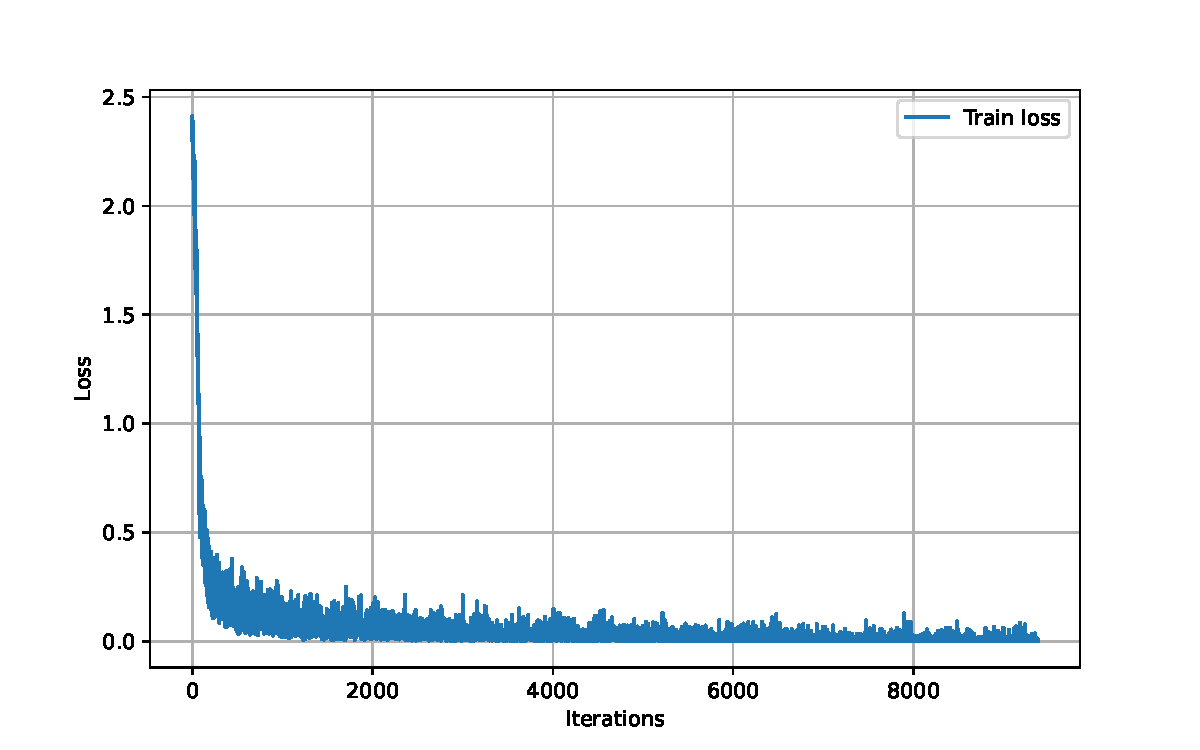
\includegraphics[width=0.6\textwidth]{ex3_3_train_loss.pdf}
  \caption{Training loss of the best Transformer model.}
  \label{fig:ex3_3_train_loss}
\end{figure}

To find the best architecture, I did a grid search over the parameters \texttt{dim}, \texttt{depth}
and \texttt{mlp\_dim}, because these are the most important parameters. I kept the number of heads
fixed at $8$, the batch size at $128$ and the number of epochs at $20$. The results are shown in
Table~\ref{tab:transformer_accuracy}. Comparing the results of the different architectures, one can
see that the accuracy is very similar for most of them. The training time however increases with the
number of dimensions. The parameter \texttt{dim} has the biggest impact on the accuracy. A bigger
dimensionality leads to better results. The depth and the MLP dimension have a smaller impact.\\
The best model had a dimension of $128$, a depth of $8$ and an MLP dimension of $128$. The accuracy
on the test set was $0.9871$. The training loss shows a lot of variance, but the model was able to
learn. The training loss is shown in Figure~\ref{fig:ex3_3_train_loss}.


\section{Generative Models}
\label{ex:4}


\subsection{Energy-Based Models}
\label{ex:4.1}

\subsubsection*{Restricted Boltzmann Machines}

\begin{task}{4.1.1}
  % In the notebook, the training algorithm refers to the pseudo-likelihood. Why is that? What are
  % the consequences regarding the training procedure?
\end{task}

Pseudo-likelihood is similar to likelihood in the sense that it is a measure of how well the model
fits the data. However, it is not a true likelihood function. Instead, it is a product of
conditional probabilities of each pixel given all other pixels. This makes it easier to compute and
is a good approximation of the true likelihood.


\begin{task}{4.1.2}
  % What is the role of the number of components, learning rate and number of iterations on the
  % performance? You can also evaluate it visually by reconstructing unseen test images.
\end{task}

\begin{figure}[ht]
  \centering
  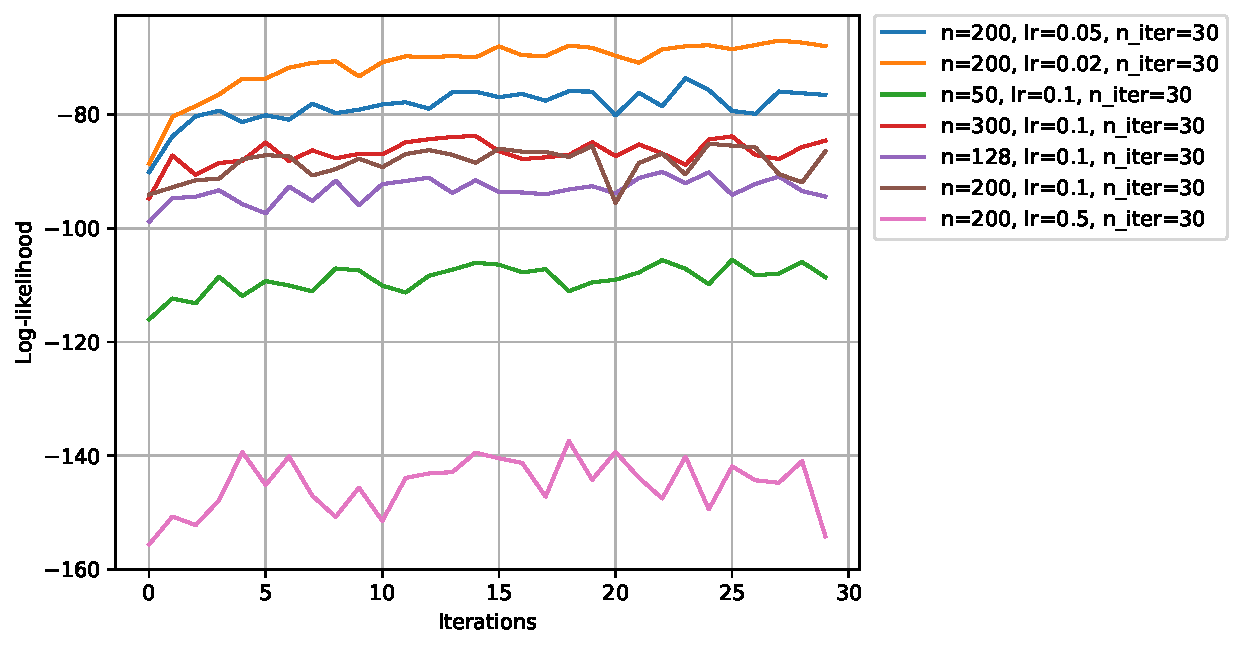
\includegraphics[width=0.9\textwidth]{ex4_1_rbm_likelihoods.pdf}
  \caption{Pseudo-likelihoods of RBM training with different parameters.}
  \label{fig:ex4_1_rbm_likelihoods}
\end{figure}

With a low learning rate, the model converges slowly which would need a higher number of iterations
to reach the same performance. On the other hand, a high learning rate can cause oscillations in the
training process. This can be seen in the variance of the pseudo-likelihood values.\\
The number of components had the biggest impact on the performance. With too few components, the
reconstructed images were blurry and did not resemble the original data. The number of iterations
needed to be big enough for the model to converge. Chosing a higher number of iterations did not
improve the performance significantly. I assumed the model to be converged based on the
pseudo-likelihood values in Figure~\ref{fig:ex4_1_rbm_likelihoods}.\\
The performance of the model was evaluated visually by reconstructing unseen test images. The best
results were achieved with $200$ components, a learning rate of $0.1$, and $30$ iterations.
Counterintuitively, the model produced more convincing results than other models that achieved a
higher pseudo-likelihood. This could be due to the fact that the pseudo-likelihood is not a perfect
measure of the model's performance.


\begin{task}{4.1.3}
  % Change the number of Gibbs sampling steps. Can you explain the result?
\end{task}

\begin{figure}[ht]
  \centering
  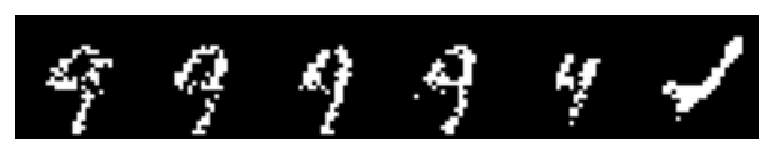
\includegraphics[width=0.9\textwidth]{ex4_1_rbm_gibbs_steps.pdf}
  \caption{Reconstructed images of a $9$ with Gibbs sampling steps. Number of Gibbs sampling steps:
    $1$, $2$, $5$, $10$, $100$, $1000$.}
  \label{fig:ex4_1_rbm_gibbs_steps}
\end{figure}

The effect of the number of Gibbs sampling steps can be seen in
Figure~\ref{fig:ex4_1_rbm_gibbs_steps}. With only one Gibbs sampling step, the model can already
reconstruct the image quite well. With more steps, the image only improves slightly. After more than
$10$ steps, the image degrades and converges to something that could resemble a different digit or
the mean of all digits. This could be related to the problem of iterated functions, where the model
converges to a fixed point.

\begin{task}{4.1.4}
  % Use the RBM to reconstruct missing parts of images. Discuss the results.
\end{task}

\begin{figure}[ht!]
  \centering
  \begin{minipage}{0.48\textwidth}
    \centering
    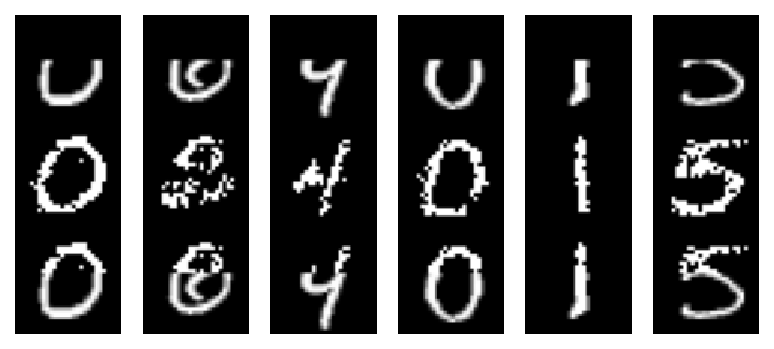
\includegraphics[width=0.9\linewidth]{ex4_1_rbm_reconstruction.pdf}
    \captionof{figure}{Top: Original images with missing parts. Middle: Reconstructed images. Bottom: Merge of original and reconstructed images.}
    \label{fig:ex4_1_rbm_reconstruction}
  \end{minipage}
  \begin{minipage}{0.48\textwidth}
    \centering
    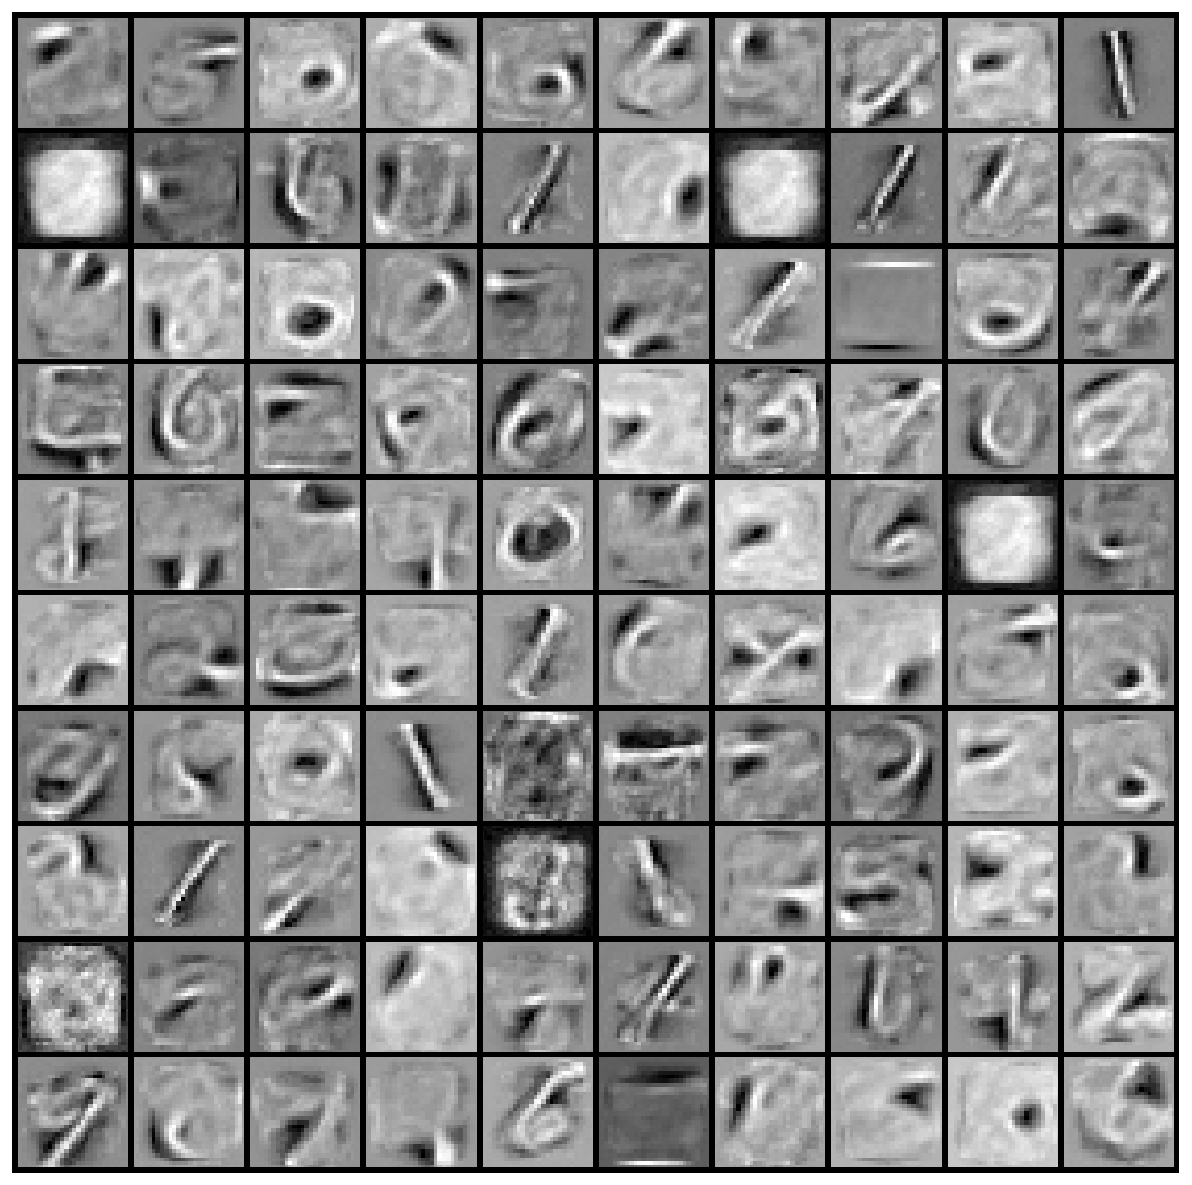
\includegraphics[width=0.9\linewidth]{ex4_1_rbm_components.pdf}
    \captionof{figure}{Components of the RBM.}
    \label{fig:ex4_1_rbm_components}
  \end{minipage}
\end{figure}

In this example, 12 rows at the top of the image were removed. The RBM is able to reconstruct some
digits better than others, as shown in Figure~\ref{fig:ex4_1_rbm_reconstruction}. Two of the
$0$-digits have decent reconstructions. The digit $1$ works particularly well, likely because of its
simple shape. The digit $9$ is falsely reconstructed as a $4$. However, the model manages to
reconstruct the digit $5$ correctly, even though it could also be seen as a $3$ with the top part
missing. In this case, the model has the most trouble with the second $0$-digit, because of the
additional stroke in the middle.


\begin{task}{4.1.5}
  % What is the effect of removing more rows in the image on the ability of the network to
  % reconstruct? What if you remove rows on different locations (top, middle...)?
\end{task}

When removing more rows, the quality of the reconstruction decreases quickly. With $16$ rows
removed, the model only manages to reconstruct about half of the digits correctly. Removing rows on
the bottom, left or right side of the image has a similar effect. With removed rows in the middle,
the model has more trouble, likely because the middle of the image contains more context than the
edges.

\vspace*{0.3cm}
\subsubsection*{Deep Boltzmann Machines}

\begin{task}{4.1.6}
  % Load the pre-trained DBM that is trained on the MNIST database. Show the filters
  % (interconnection weights) extracted from the previously trained RBM (cf. supra) and the DBM,
  % what is the difference? Can you explain the difference between filters of the first and second
  % layer of the DBM?
\end{task}

\begin{figure}[ht]
  \centering
  \begin{subfigure}{0.49\textwidth}
    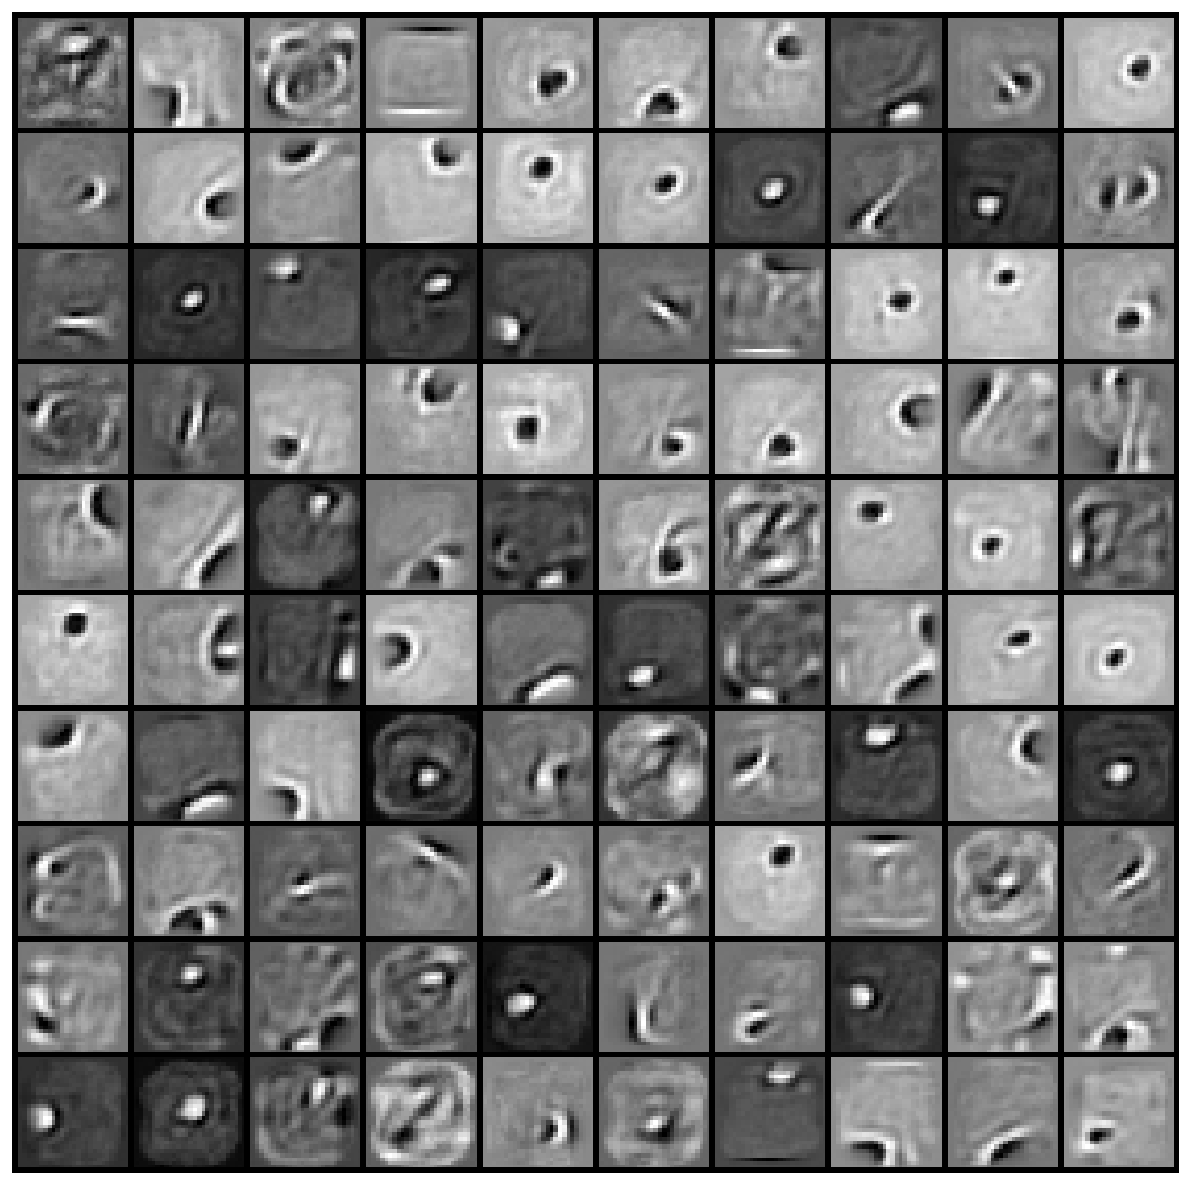
\includegraphics[width=\textwidth]{ex4_1_dbm_components_1.pdf}
    \caption{First layer}
    \label{fig:ex4_1_dbm_components_1}
  \end{subfigure}
  \begin{subfigure}{0.49\textwidth}
    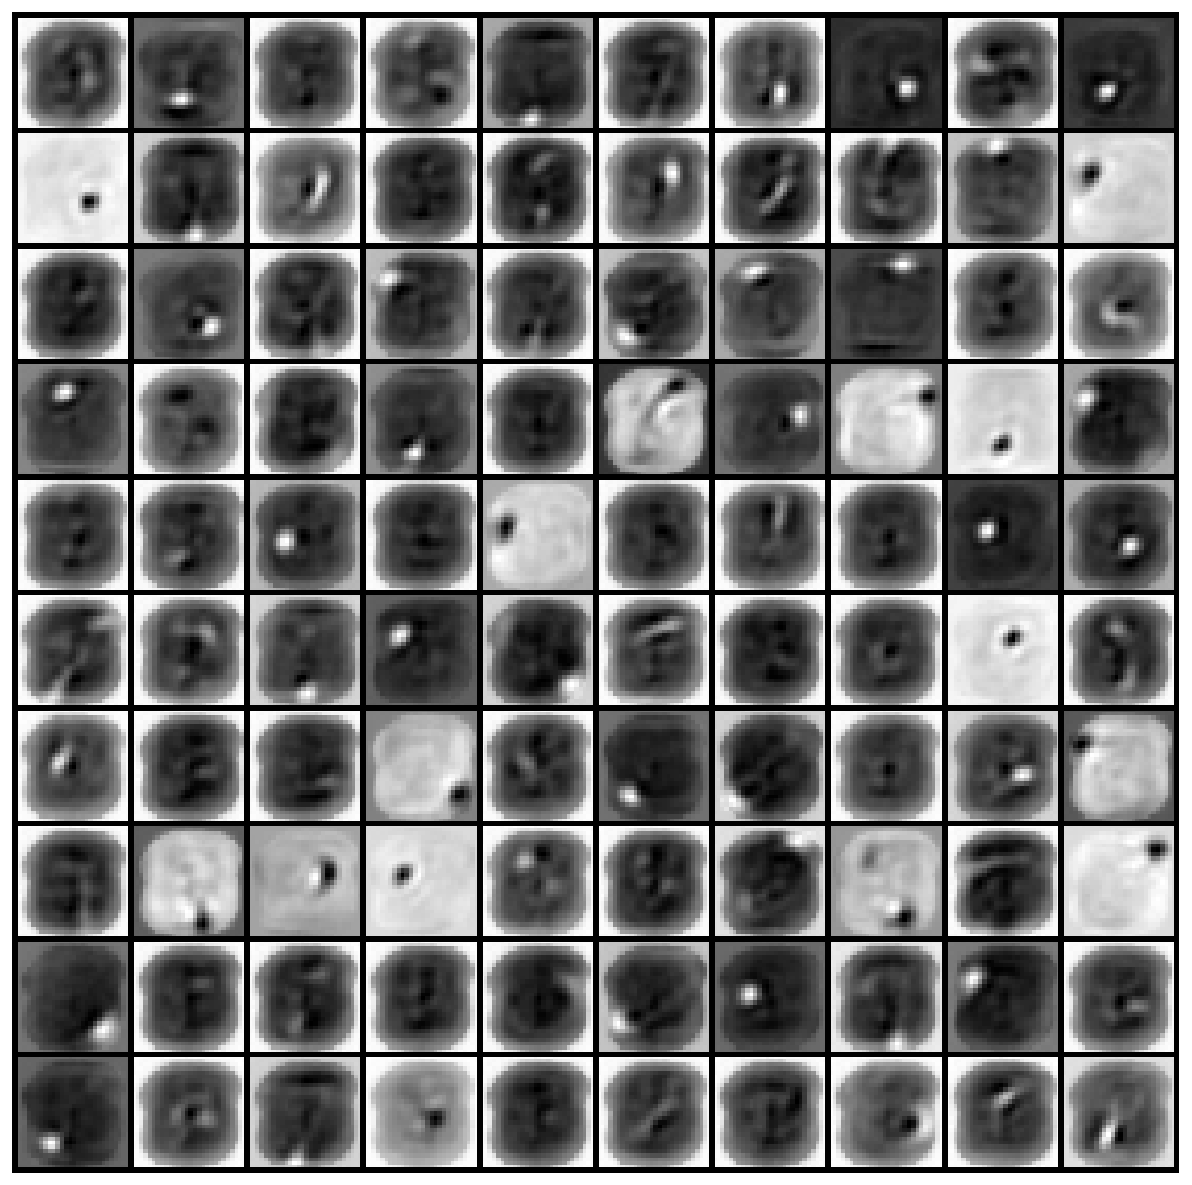
\includegraphics[width=\textwidth]{ex4_1_dbm_components_2.pdf}
    \caption{Second layer}
    \label{fig:ex4_1_dbm_components_2}
  \end{subfigure}
  \caption{Components of the DBM.}
  \label{fig:ex4_1_dbm_components}
\end{figure}

Comparing the components of the RBM (see Figure~\ref{fig:ex4_1_rbm_components}) and the first layer
of the DBM (see Figure~\ref{fig:ex4_1_dbm_components_1}), the components of the RBM have many more
lines and structures that resemble the digits. Most of them look unstructured and seem to focus more
on the edges, because of dark lines directly next to white lines. The components of the DBM on the
other hand often have a dark background with a bright center or vice versa. This could be related to
the fact that the DBM has more layers and every component can focus on more abstract features.\\
The majority of the components of the second layer have white edges and a dark center, as shown in
Figure~\ref{fig:ex4_1_dbm_components_2}. Many of them also have a spot in the middle, but it is not
as pronounced as in the first layer. Overall, the components of the second layer have much more
contrast than the first layer.


\begin{task}{4.1.7}
  % Sample new images from the DBM. Is the quality better than the RBM from the previous exercise?
  % Explain.
\end{task}

\begin{figure}[ht]
  \centering
  \begin{subfigure}{0.49\textwidth}
    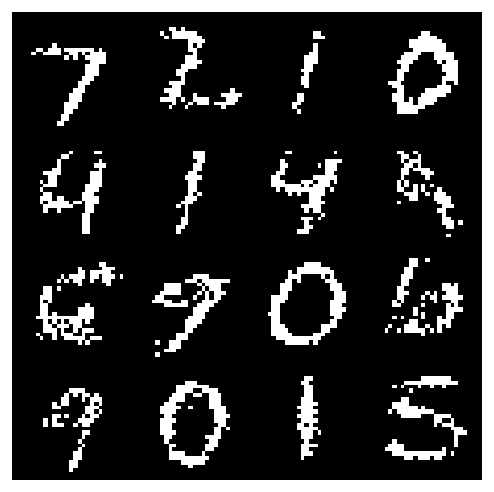
\includegraphics[width=\textwidth]{ex4_1_rbm_samples.pdf}
    \caption{RBM}
    \label{fig:ex4_1_rbm_samples}
  \end{subfigure}
  \begin{subfigure}{0.49\textwidth}
    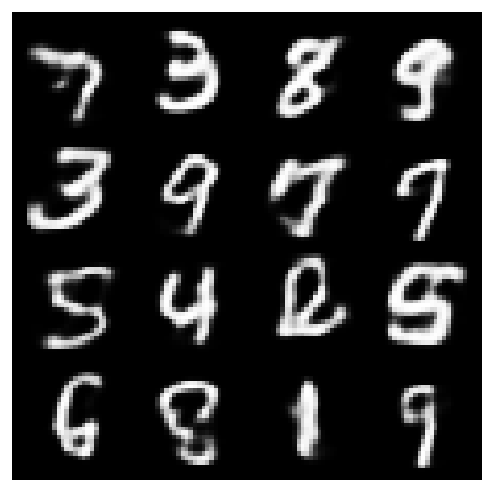
\includegraphics[width=\textwidth]{ex4_1_dbm_samples.pdf}
    \caption{DBM}
    \label{fig:ex4_1_dbm_samples}
  \end{subfigure}
  \caption{Samples generated after 1 Gibbs sampling step.}
  \label{fig:ex4_1_samples}
\end{figure}

The samples generated by the RBM and the DBM after 1 Gibbs sampling step are shown in
Figure~\ref{fig:ex4_1_samples}. The samples of the DBM are of higher quality than the samples of the
RBM, because they resemble digits more closely and have less artifacts. The biggest difference is
that the RBM only produces binary pixel values, while the digits of the DBM have continuous edges,
like anti-aliasing was applied. Also, the structure of the digits is more consistent in the DBM
samples.


\subsection{Generator and Discriminator in the Ring}
\label{ex:4.2}

\begin{task}{4.2.1}
  % Explain the different losses and results in the context of the GAN framework.
\end{task}

The loss of the generator measures how good the generator is at fooling the discriminator. The
generator tries to minimize this loss by generating samples that are similar to the real data. The
loss of the discriminator measures how good the discriminator is at distinguishing between real and
fake samples. The discriminator tries to minimize this loss by correctly classifying the samples.


\begin{task}{4.2.2}
  % What would you expect if the discriminator performs proportionally much better than the
  % generator?
\end{task}

If the discriminator performs much better than the generator, the generator will have a hard time
fooling the discriminator. This could lead to mode collapse, where the generator only produces a few
different samples. The generator will not be able to learn from the feedback of the discriminator.


\begin{task}{4.2.3}
  % Discuss and illustrate the convergence and stability of GANs.
\end{task}

The losses of the generator and discriminator during training are shown in
Figure~\ref{fig:ex4_2_gan_loss}. In the optimal case, both losses should converge to a low value, so
that the generator and discriminator reach an equilibrium. The losses should be balanced, so that
the generator can learn from the feedback of the discriminator. In this case, the losses of the
generator increase. However, this does not mean that the generator is getting worse, because the
discriminator is also getting better.\\
If the losses of the generator and discriminator are not balanced, the generator will not be able to
learn from the feedback of the discriminator. This could lead to mode collapse, where the generator
only produces a few different samples.


\begin{task}{4.2.4}
  % Explore the latent space and discuss.
\end{task}

A batch of random samples generated by the GAN is shown in Figure~\ref{fig:ex4_2_samples}. Most of
the samples resemble the digit $0$. The structure of the digits is clear for about half of the
samples. The model seems to prefer round shapes, as there are only a few samples that could be
interpreted as a $4$ or $7$ and none that could be interpreted as a $1$. Also, all samples have
a noisy background, some more than others.


\begin{task}{4.2.5}
  % Try the CNN-based backbone and discuss.
\end{task}

\begin{figure}[ht]
  \centering
  \begin{subfigure}{0.49\textwidth}
    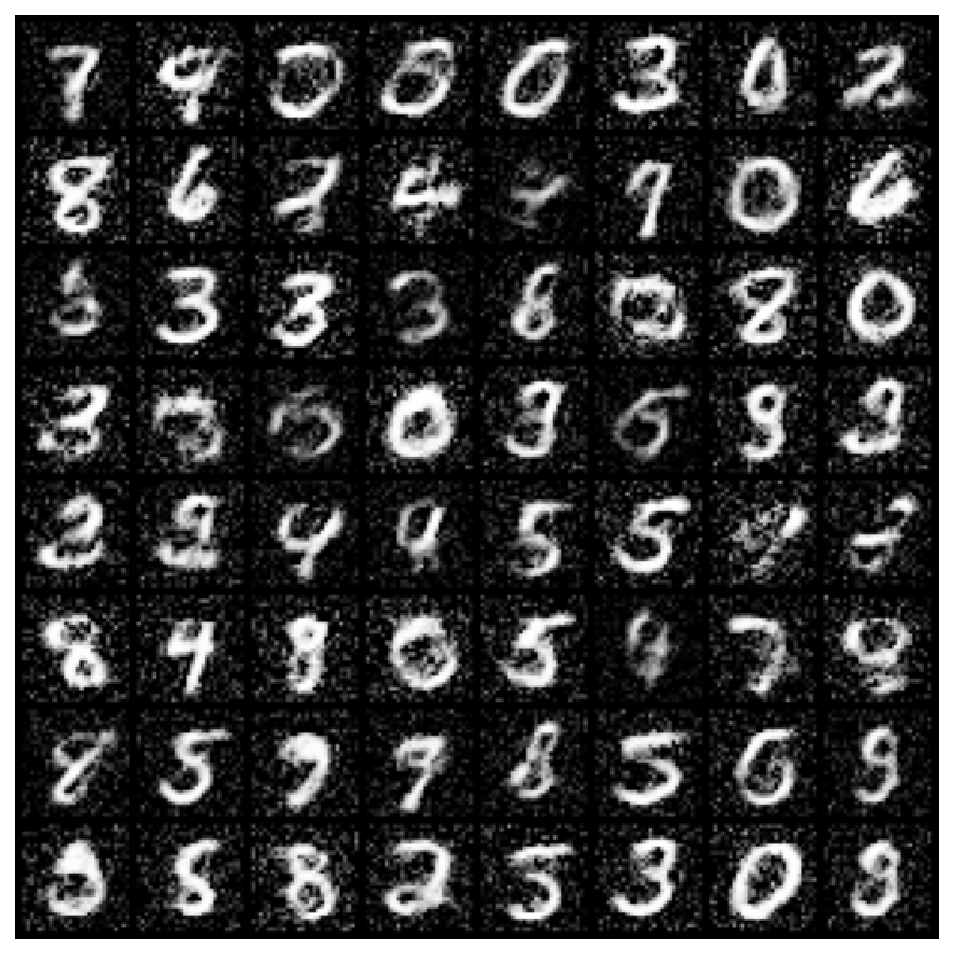
\includegraphics[width=\textwidth]{ex4_2_samples_vanilla.pdf}
    \caption{Feedforward backbone}
    \label{fig:ex4_2_samples_vanilla}
  \end{subfigure}
  \begin{subfigure}{0.49\textwidth}
    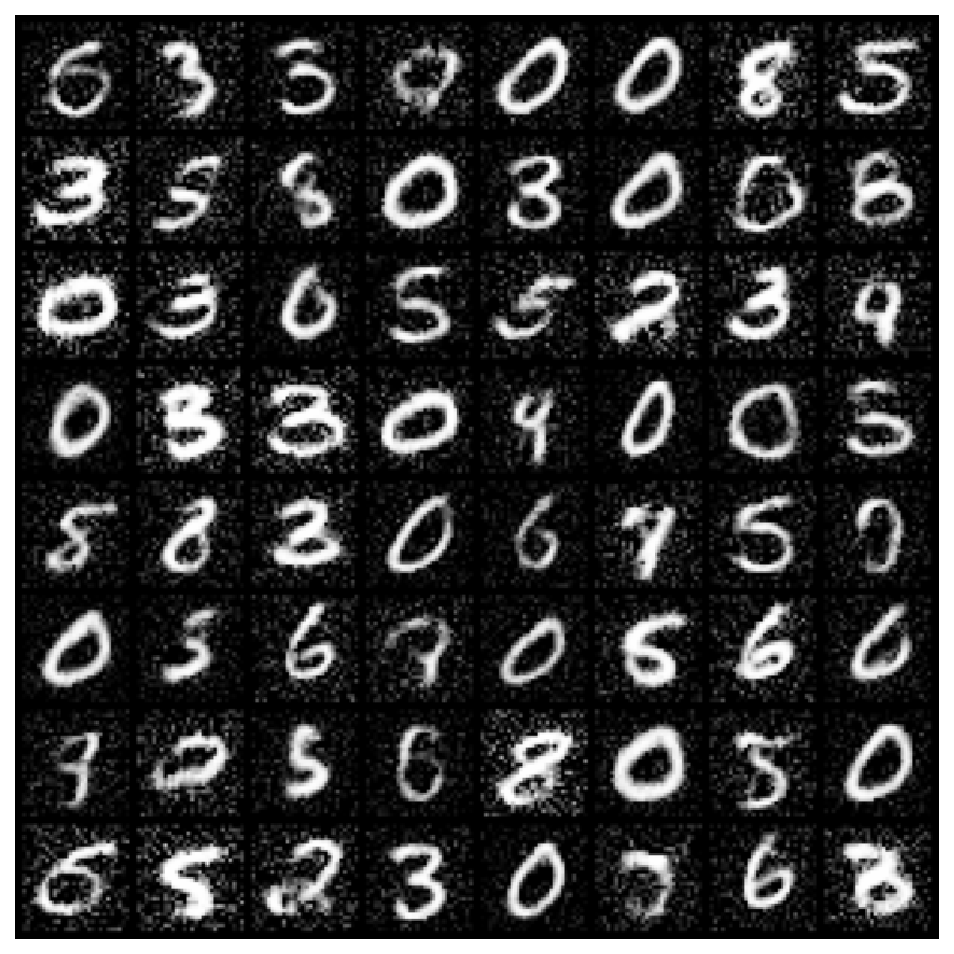
\includegraphics[width=\textwidth]{ex4_2_samples_cnn.pdf}
    \caption{CNN backbone}
    \label{fig:ex4_2_samples_cnn}
  \end{subfigure}
  \caption{Samples generated by the GAN with different backbones.}
  \label{fig:ex4_2_samples}
\end{figure}

A comparison of the samples generated by the GAN with the different backbones is shown in
Figure~\ref{fig:ex4_2_samples}. In general, the samples generated by the CNN backbone are of higher
quality. The structure of the digits is clearer and the background is less noisy. There are only a
few samples that are hardly recognizable as digits. The CNN backbone also prefers round shapes and
the digit $0$ is also the most common digit.


\begin{task}{4.2.6}
  % What are the advantages and disadvantages of GAN-models compared to other generative models,
  % e.g. the auto-encoder family or diffusion models? Think about the conceptual aspects, the
  % quality of the results, the training considerations, etc.
\end{task}

The main advantage of GANs is that they can generate samples that are very realistic, due to the
adversarial training. However, GANs are hard to train and can be unstable. They are also prone to
mode collapse, like described above. Auto-encoders are easier to train and can also be used for
dimensionality reduction. However, they are not as good at generating realistic samples. Diffusion
models are also good at generating realistic samples, but they need longer to train. They are also
harder to understand than GANs.



\subsection{An Auto-Encoder With a Touch}
\label{ex:4.3}

\begin{task}{4.3.1}
  % In practice, the model does not maximize the log-likelihood but another metric. Which one? Why
  % is that and how does it work?
\end{task}

The model maximizes the evidence lower bound (ELBO) instead of the log-likelihood. The ELBO is the
sum of the (negative) reconstruction error and the Kullback-Leibler divergence between the latent
distribution and the prior distribution. The reconstruction error expresses how good the model is at
reconstructing the input data. The KL-divergence measures how much information is lost when the
latent distribution is approximated by the prior distribution.\\
The ELBO is used because it is easier to optimize than the log-likelihood. Also, the KL-divergence
term acts as a regularizer that prevents the model from overfitting.


\begin{task}{4.3.2}
  % In particular, what similarities and differences do you see when compared with stacked
  % auto-encoder from the previous assignment? What is the metric for the reconstruction error in
  % each case?
\end{task}

The main difference between the stacked auto-encoder and the VAE is that the VAE uses a
probabilistic approach to model the latent space. This allows the VAE to generate new samples by
sampling from the latent space. The stacked auto-encoder uses cross entropy and the VAE uses binary
cross entropy as the metric for the reconstruction error.


\begin{task}{4.3.3}
  % Explore the latent space using the provided code and discuss what you observe.
\end{task}

\begin{figure}[t]
  \centering
  \begin{minipage}{0.6\textwidth}
    \centering
    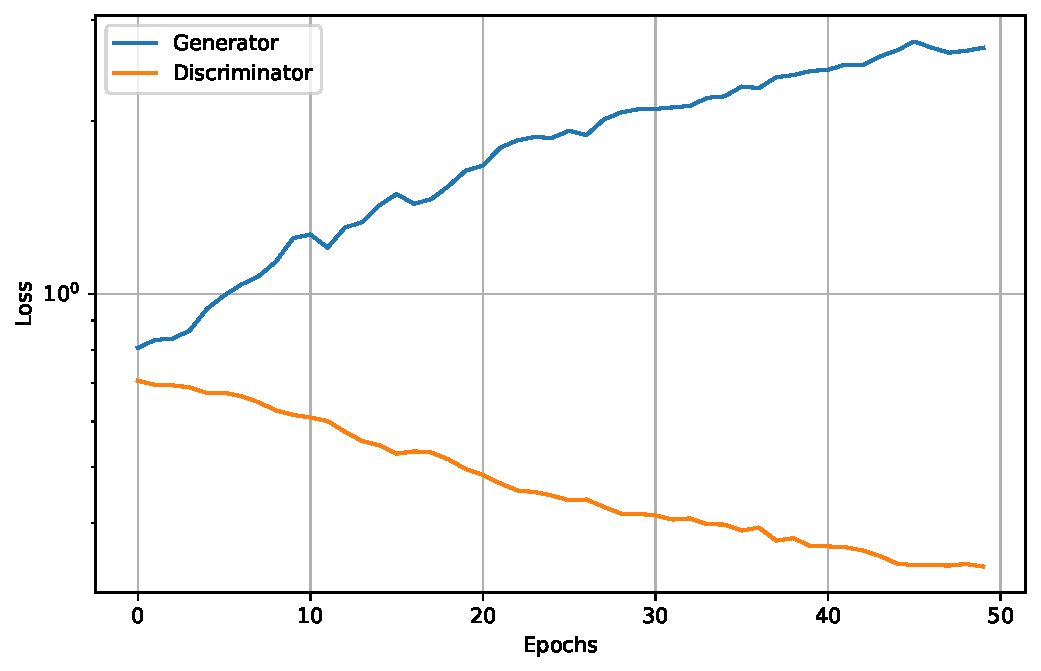
\includegraphics[width=0.9\linewidth]{ex4_2_gan_loss.pdf}
    \captionof{figure}{Losses of the generator and discriminator during training.}
    \label{fig:ex4_2_gan_loss}
  \end{minipage}
  \begin{minipage}{0.39\textwidth}
    \centering
    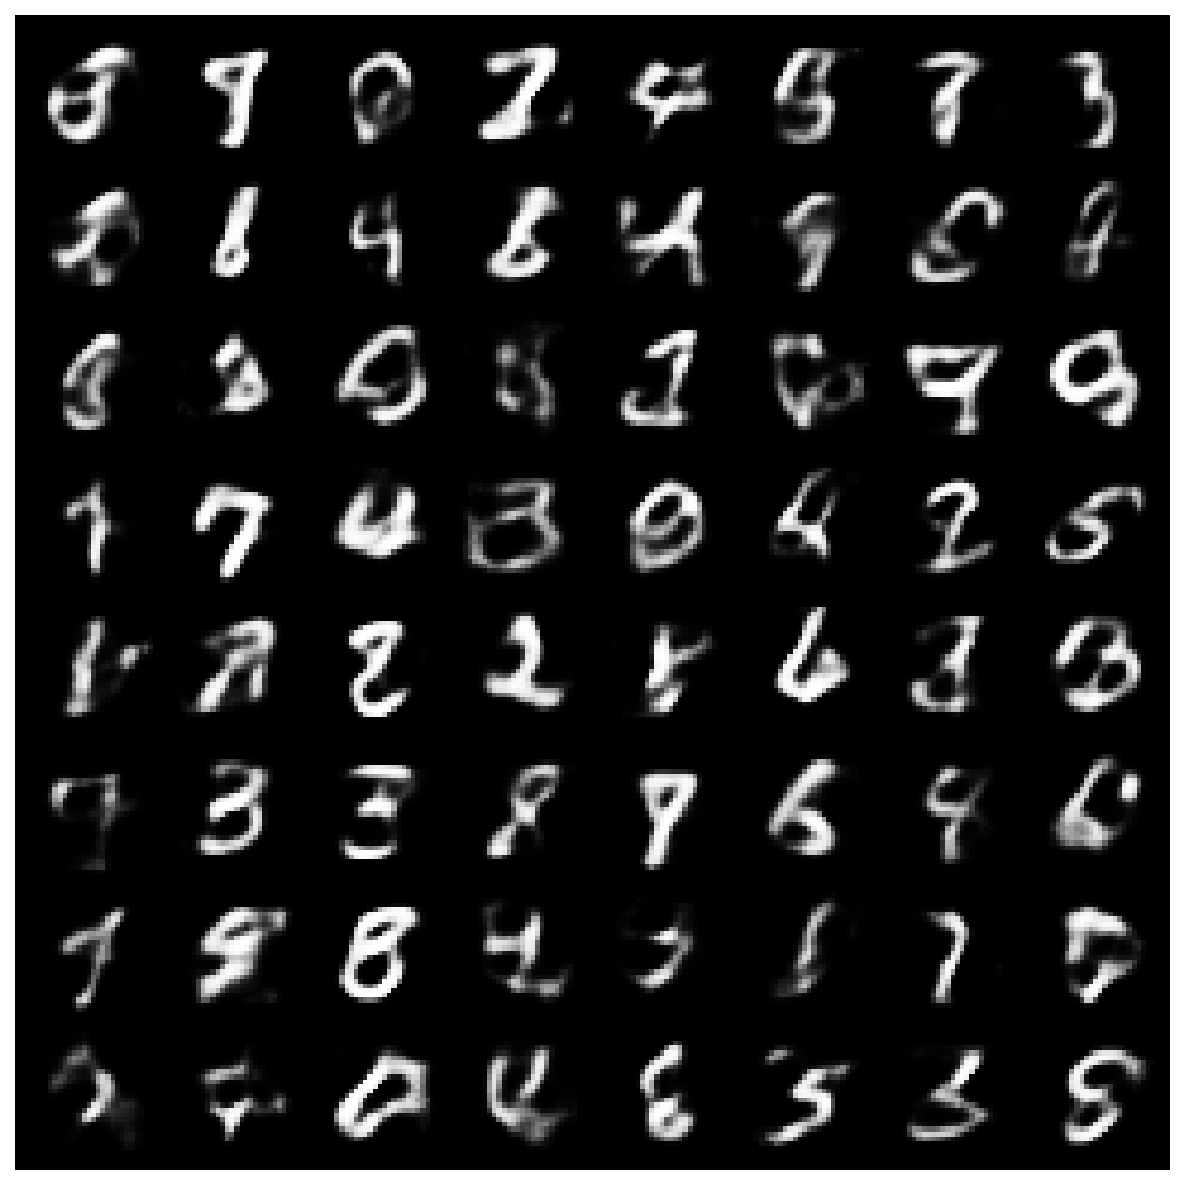
\includegraphics[width=0.9\linewidth]{ex4_3_samples.pdf}
    \captionof{figure}{Random samples from the latent space of the VAE.}
    \label{fig:ex4_3_samples}
  \end{minipage}
\end{figure}

I trained the VAE with latent-space dimension $300$ and middle layer dimension $1024$ for $100$
epochs. The samples from the latent space are shown in Figure~\ref{fig:ex4_3_samples}. One can tell
that they are supposed to be digits, but only a few of them have a clear structure. There are some
samples that are not recognizable as digits at all. Others can be seen as a digit, but are not
clearly defined. A big majority of the outputs look like the digit $8$. Also, there is no sample
that is clearly a $0$-digit. I consider this as counterintuitive, because of its simple shape.


\begin{task}{4.3.4}
  % Compare the generation mechanism to GANs. You may optionally want to consider similar backbones
  % for a fair comparison. What are the advantages and disadvantages?
\end{task}

The VAE generates samples by sampling from the latent space, while the GAN generates samples by
feeding random noise through the generator. The VAE has the advantage that it can generate samples
from the latent space, while the GAN can only generate samples from the input space. This makes the
VAE more interpretable, because you can see how the latent space is structured. The GAN has the
advantage that it can generate more realistic samples, because it is trained to fool the
discriminator.


\end{document}
